% Copyright (c) 2022 by Lars Spreng
% Content Copyright (c) 2023 by Garvin Lab & Bensmaia Lab & Ronghao Zhang (MIT License)
% This work is licensed under the Creative Commons Attribution 4.0 International License. 
% To view a copy of this license, visit http://creativecommons.org/licenses/by/4.0/ or send a letter to Creative Commons, PO Box 1866, Mouhttps://www.overleaf.com/project/63a9d5f62ffa2461bb5e8a9dntain View, CA 94042, USA.

%~~~~~~~~~~~~~~~~~~~~~~~~~~~~~~~~~~~~~~~~~~~~~~~~~~~~~~~~~~~~~~~~~~~~~~~~~~~~~~
% You can add your packages and commands to the loadslides.tex file. 
% The files in the folder "styles" can be modified to change the layout and design of your slides.
% I have included examples on how to use the template below. 
% Some of it these examples are taken from the Metropolis template.
%~~~~~~~~~~~~~~~~~~~~~~~~~~~~~~~~~~~~~~~~~~~~~~~~~~~~~~~~~~~~~~~~~~~~~~~~~~~~~~

\documentclass[
11pt,notheorems,hyperref={pdfauthor=whatever}
]{beamer}


% Copyright (c) 2022 by Lars Spreng
% This work is licensed under the Creative Commons Attribution 4.0 International License. 
% To view a copy of this license, visit http://creativecommons.org/licenses/by/4.0/ or send a letter to Creative Commons, PO Box 1866, Mountain View, CA 94042, USA.

%~~~~~~~~~~~~~~~~~~~~~~~~~~~~~~~~~~~~~~~~~~~~~~~~~~~~~~~~~~~~~~~~~~~~~~~~~~~~~~
% Add your packages and commands to this file
%~~~~~~~~~~~~~~~~~~~~~~~~~~~~~~~~~~~~~~~~~~~~~~~~~~~~~~~~~~~~~~~~~~~~~~~~~~~~~~

%~~~~~~~~~~~~~~~~~~~~~~~~~~~~~~~~~~~~~~~~~~~~~~~~~~~~~~~~~~~~~~~~~~~~~~~~~~~~~~
\RequirePackage{palatino}
\RequirePackage[utf8]{inputenc}
\RequirePackage[T1]{fontenc}

\usefonttheme{serif}
\usepackage{styles/elegantmacros}
\usefolder{styles}
\usetheme[style=blue]{elegant}

\newcommand{\makepart}[1]{ % For convenience
\part{#1} \frame{\partpage}
}

\usepackage{setspace}
\onehalfspacing

%~~~~~~~~~~~~~~~~~~~~~~~~~~~~~~~~~~~~~~~~~~~~~~~~~~~~~~~~~~~~~~~~~~~~~~~~~~~~~~

%~~~~~~~~~~~~~~~~~~~~~~~~~~~~~~~~~~~~~~~~~~~~~~~~~~~~~~~~~~~~~~~~~~~~~~~~~~~~~~
% Figures
\RequirePackage{booktabs}
\RequirePackage{colortbl}
\RequirePackage{ragged2e}
\RequirePackage{schemabloc}
%\RequirePackage{natbib}
\RequirePackage{caption}
\RequirePackage{subcaption}
\RequirePackage{tabularx}
\RequirePackage{array}
\RequirePackage{multirow}
\usepackage{graphicx}
\usepackage[bibstyle=apa]{biblatex}
\addbibresource{bibliography.bib}
\newcolumntype{Y}{>{\centering\arraybackslash}X}

%~~~~~~~~~~~~~~~~~~~~~~~~~~~~~~~~~~~~~~~~~~~~~~~~~~~~~~~~~~~~~~~~~~~~~~~~~~~~~~

%~~~~~~~~~~~~~~~~~~~~~~~~~~~~~~~~~~~~~~~~~~~~~~~~~~~~~~~~~~~~~~~~~~~~~~~~~~~~~~
% Figures
\RequirePackage{wrapfig}
\RequirePackage{pgfplots}
\RequirePackage{graphicx}
\RequirePackage{adjustbox}
\RequirePackage{environ}
\pgfplotsset{compat=1.18}

\makeatletter
\newsavebox{\measure@tikzpicture}
\NewEnviron{scaletikzpicturetowidth}[1]{%
  \def\tikz@width{#1}%
  \def\tikzscale{1}\begin{lrbox}{\measure@tikzpicture}%
  \BODY
  \end{lrbox}%
  \pgfmathparse{#1/\wd\measure@tikzpicture}%
  \edef\tikzscale{\pgfmathresult}%
  \BODY
}
\makeatother
%~~~~~~~~~~~~~~~~~~~~~~~~~~~~~~~~~~~~~~~~~~~~~~~~~~~~~~~~~~~~~~~~~~~~~~~~~~~~~~

%~~~~~~~~~~~~~~~~~~~~~~~~~~~~~~~~~~~~~~~~~~~~~~~~~~~~~~~~~~~~~~~~~~~~~~~~~~~~~~
% Maths 
\RequirePackage{textcomp}
\RequirePackage{amsmath} 
\RequirePackage{amsthm}
\RequirePackage{mathtools}
%\RequirePackage{bbm}
%\RequirePackage{algorithm}
%\RequirePackage[osf,sc]{mathpazo}
%\RequirePackage{pifont}
%\newcommand{\xmark}{\ding{55}}%
%\numberwithin{equation}{section}
\DeclareMathOperator*{\argmax}{arg\,max}
\DeclareMathOperator*{\argmin}{arg\,min}

\setbeamertemplate{theorems}[numbered] % to number

\theoremstyle{definition}
\newtheorem{fact}{Fact}[section]
\newtheorem{examp}{Example}[section]

\theoremstyle{plain}
\newtheorem{definition}{Definition}[section]
\newtheorem{proposition}{Proposition}
\newtheorem{theorem}{Theorem}
\newtheorem{assumption}{Assumption}

\providecommand{\H}{\mathscr{H}}      
\providecommand{\E}{\mathbb{E}}
\makeatletter
\def\munderbar#1{\underline{\sbox\tw@{$#1$}\dp\tw@\z@\box\tw@}}
\makeatother

%~~~~~~~~~~~~~~~~~~~~~~~~~~~~~~~~~~~~~~~~~~~~~~~~~~~~~~~~~~~~~~~~~~~~~~~~~~~~~~
 % Loads packages and some defined commands

%Path relative to the main .tex file 
\graphicspath{ {./images/} }

\title[
% Text entered here will appear in the bottom middle
]{Oral Presentation for Ronghao's Undergraduate Research}

\subtitle{Keywords: Renal Physiology; Transcriptomics; Computational Neuroscience}

\author[
% Text entered here will appear in the bottom left corner
]{
    Ronghao (Luke) Zhang
}

\institute{
    Department of Physiology and Biophysics, \\
    School of Medicine, \\
    Case Western Reserve University}
\date{\today}

\begin{document}

% Generate title page
{
\setbeamertemplate{footline}{} 
\begin{frame}
  \titlepage
\end{frame}
}
\addtocounter{framenumber}{-1}

% You can declare different parts as a parentof sections: INDEX GOES HERE
\begin{frame}{Part I: Renal Physiology}
    \tableofcontents[part=1]
\end{frame}
\begin{frame}{Part II: Computational Neuroscience}
    \tableofcontents[part=2]
\end{frame}

%% PART I: RENAL PHYSIOLOGY ----------
\makepart{Renal Physiology}

%%% Significance of Doing Renal Physiology
\begin{frame}{Why Renal Physiology and Hypertension?}{Significance of Projects}
    \begin{itemize}
        \item Hypertension is the leading cause of health deficiencies.
        \item Dietary fructose consumption has increased by \textbf{20 times} in 2010 compared to that in 1970. 
        \item Fructose metabolism in the kidney can affect blood pressure homeostatsis and cause hypertension over time. 
    \end{itemize}
    \begin{table}
        \renewcommand{\tablename}{Table 1}
        \caption{Dietary fructose consumption in the past decades}
        \begin{tabular}{@{} lr @{}}
          \toprule
          Year & Fructose Consumption \\
          \midrule
          1970 & <\,2 lbs/person/yr\\
          2010 & >\,40 lbs/person/yr\\
          \bottomrule
        \end{tabular}
    \end{table}
\end{frame}

%%% Garvin Project 1: Fructose & Expression of Aldosterone-Response Genes
\section{Fructose \& Expression of Aldosterone-Response Genes}
\begin{frame}{}{Contribution}
\begin{itemize}
    \item \textbf{Duration:} 
    \begin{itemize}
        \item Janurary 2022 - Present
    \end{itemize}
    \item \textbf{Keywords:} 
    \begin{itemize}
        \item Transcriptomics; Epithelial transport in kidney
    \end{itemize}
    \item \textbf{Publication:} 
    \begin{itemize}
        \item Submitted an abstract as the first author to the American Physiology Summit
    \end{itemize}
    \item \textbf{Involvement:}
    \begin{itemize}
        \item Designing techniques and approaches
        \item Multi-disciplinary collaboration
        \item Sample collection and cataloguing
        \item Data analysis and interpretation
        \item Dissemination and presentation of results
    \end{itemize}
\end{itemize}
\end{frame}

\subsection{Introduction}
\begin{frame}
    \begin{columns}[T,onlytextwidth]
        \column{0.6\textwidth}
          \begin{itemize}
            \item The proximal tubule (PT) reabsorbs fructose via a Na-dependent mechanism \cite{gonzalez2019sglt5}.
            \begin{itemize}
                \item SGLT5, \textit{Slc5a10}
            \end{itemize}
            \item Reabsorbed fructose increases the epithelial transport in the PT via Angiotensin II-related mechanism \cite{gonzalez2017angii}.
            \item Renin Angiotensin Aldosterone System (RAAS)
            \item To test the effect of fructose on other segments of the nephrons
            \begin{itemize}
                \item Aldosterone-Sensitive Distal Tubule (ASDT) 
            \end{itemize}
            \item \textbf{Hypothesis:} \textit{fructose metabolism in PT could affect aldosterone signaling in the distal tubule of rats fed a high-salt diet.}
          \end{itemize}

        \column{0.4\textwidth}
        \begin{figure}[h]
            \renewcommand{\figurename}{Figure 1}
            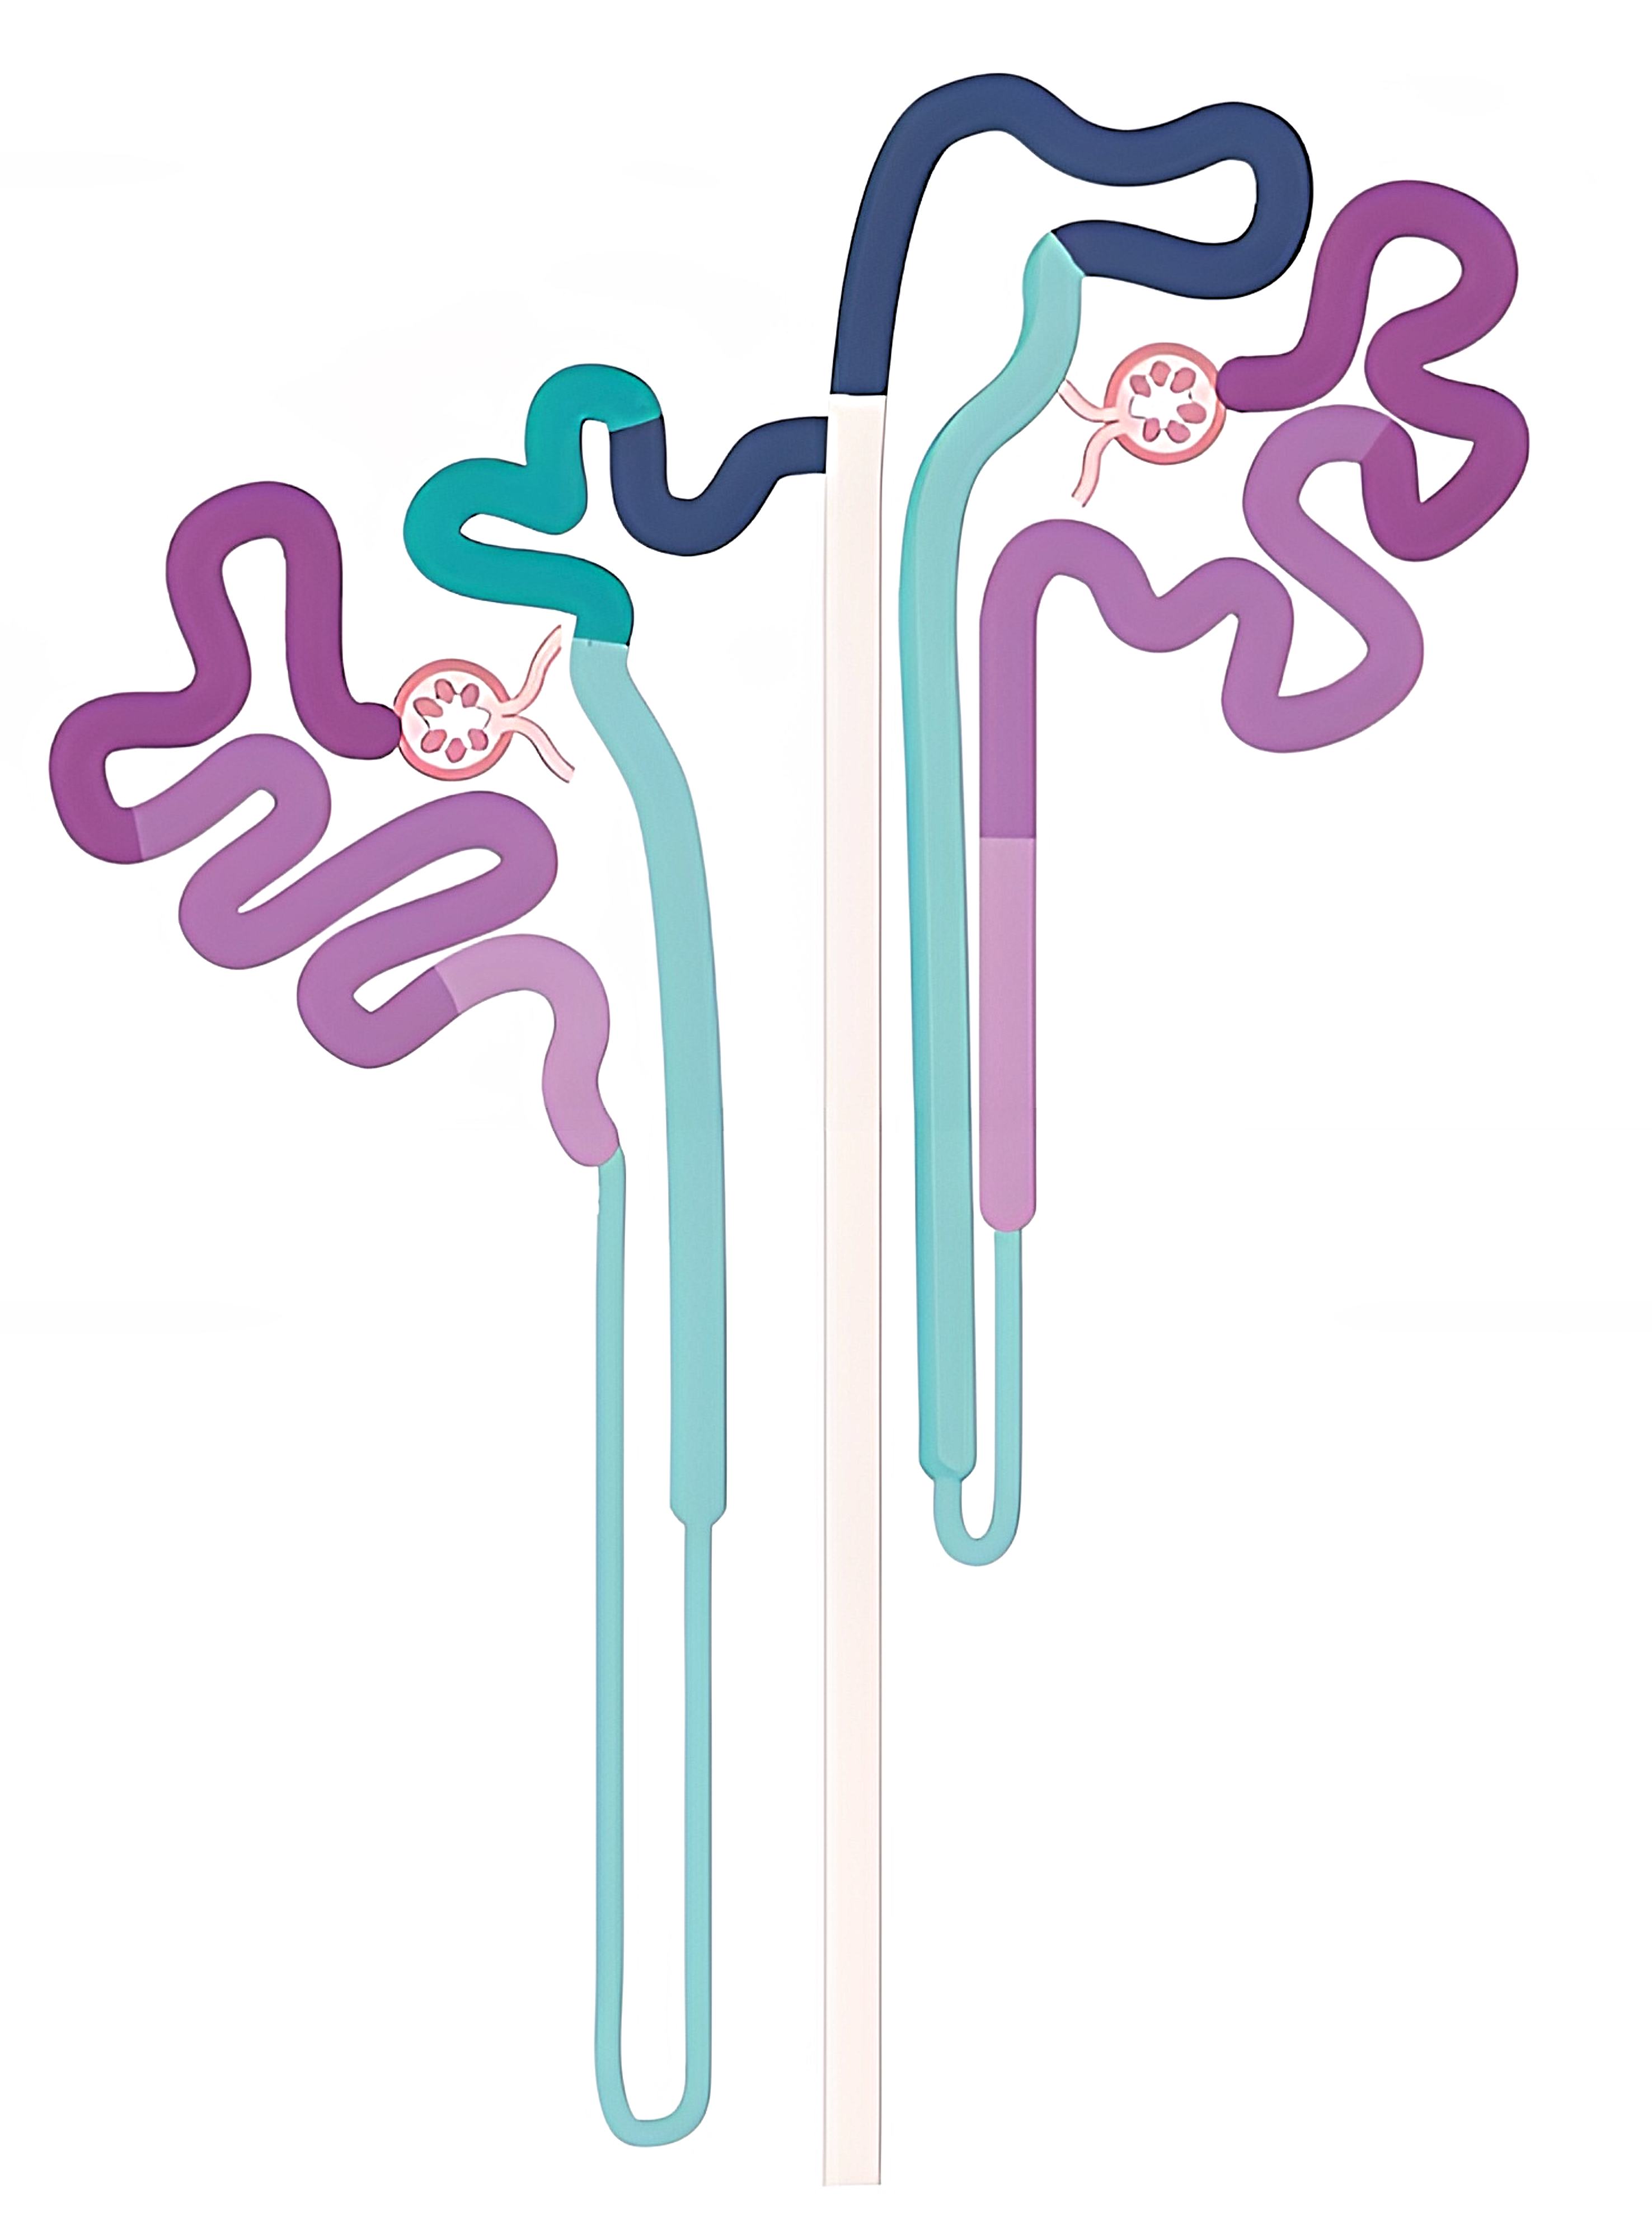
\includegraphics [scale=0.045] {AldoFruc_Nephron.jpg} 
            \caption{A diagram of superficial and juxtamedullary nephron \cite{schnell2022nephron}}
        \end{figure}
    \end{columns}
\end{frame}

\subsection{Methodology}
\begin{frame}
    \framesubtitle{Methodology: mRNA Sample Collection and Sequencing}
    \begin{figure}
        \centering
        \begin{subfigure}[b]{0.3\textwidth}
            \centering
            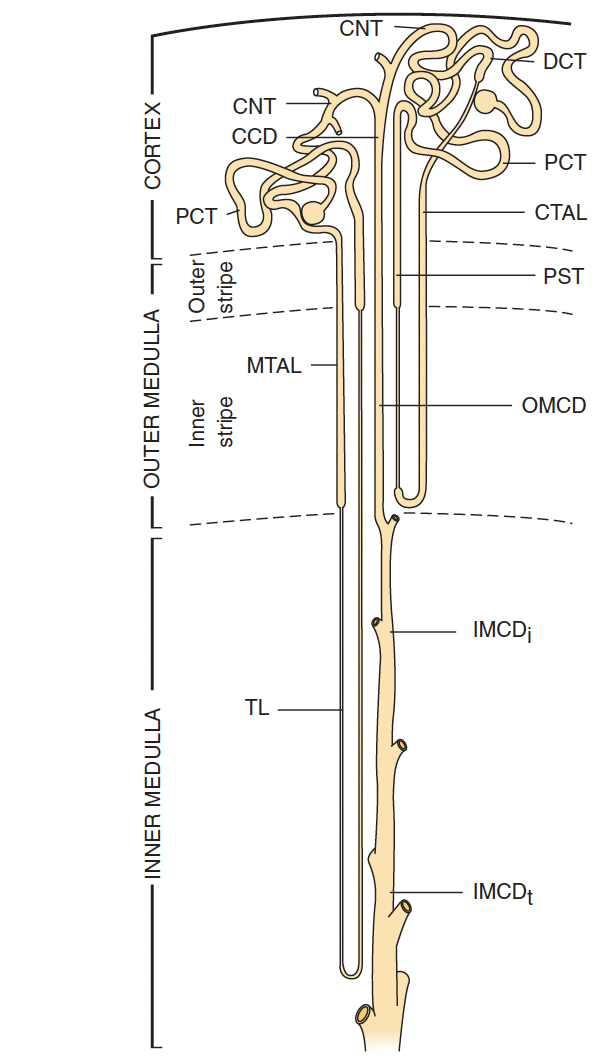
\includegraphics[scale=0.39]{AldoFruc_CortexCollection.jpg}
            \caption{Location of PT \& ADST \cite{taal2011brenner}}
            \label{fig: Location of PT and ADST}
        \end{subfigure}
        \begin{subfigure}[b]{0.3\textwidth}
            \centering
            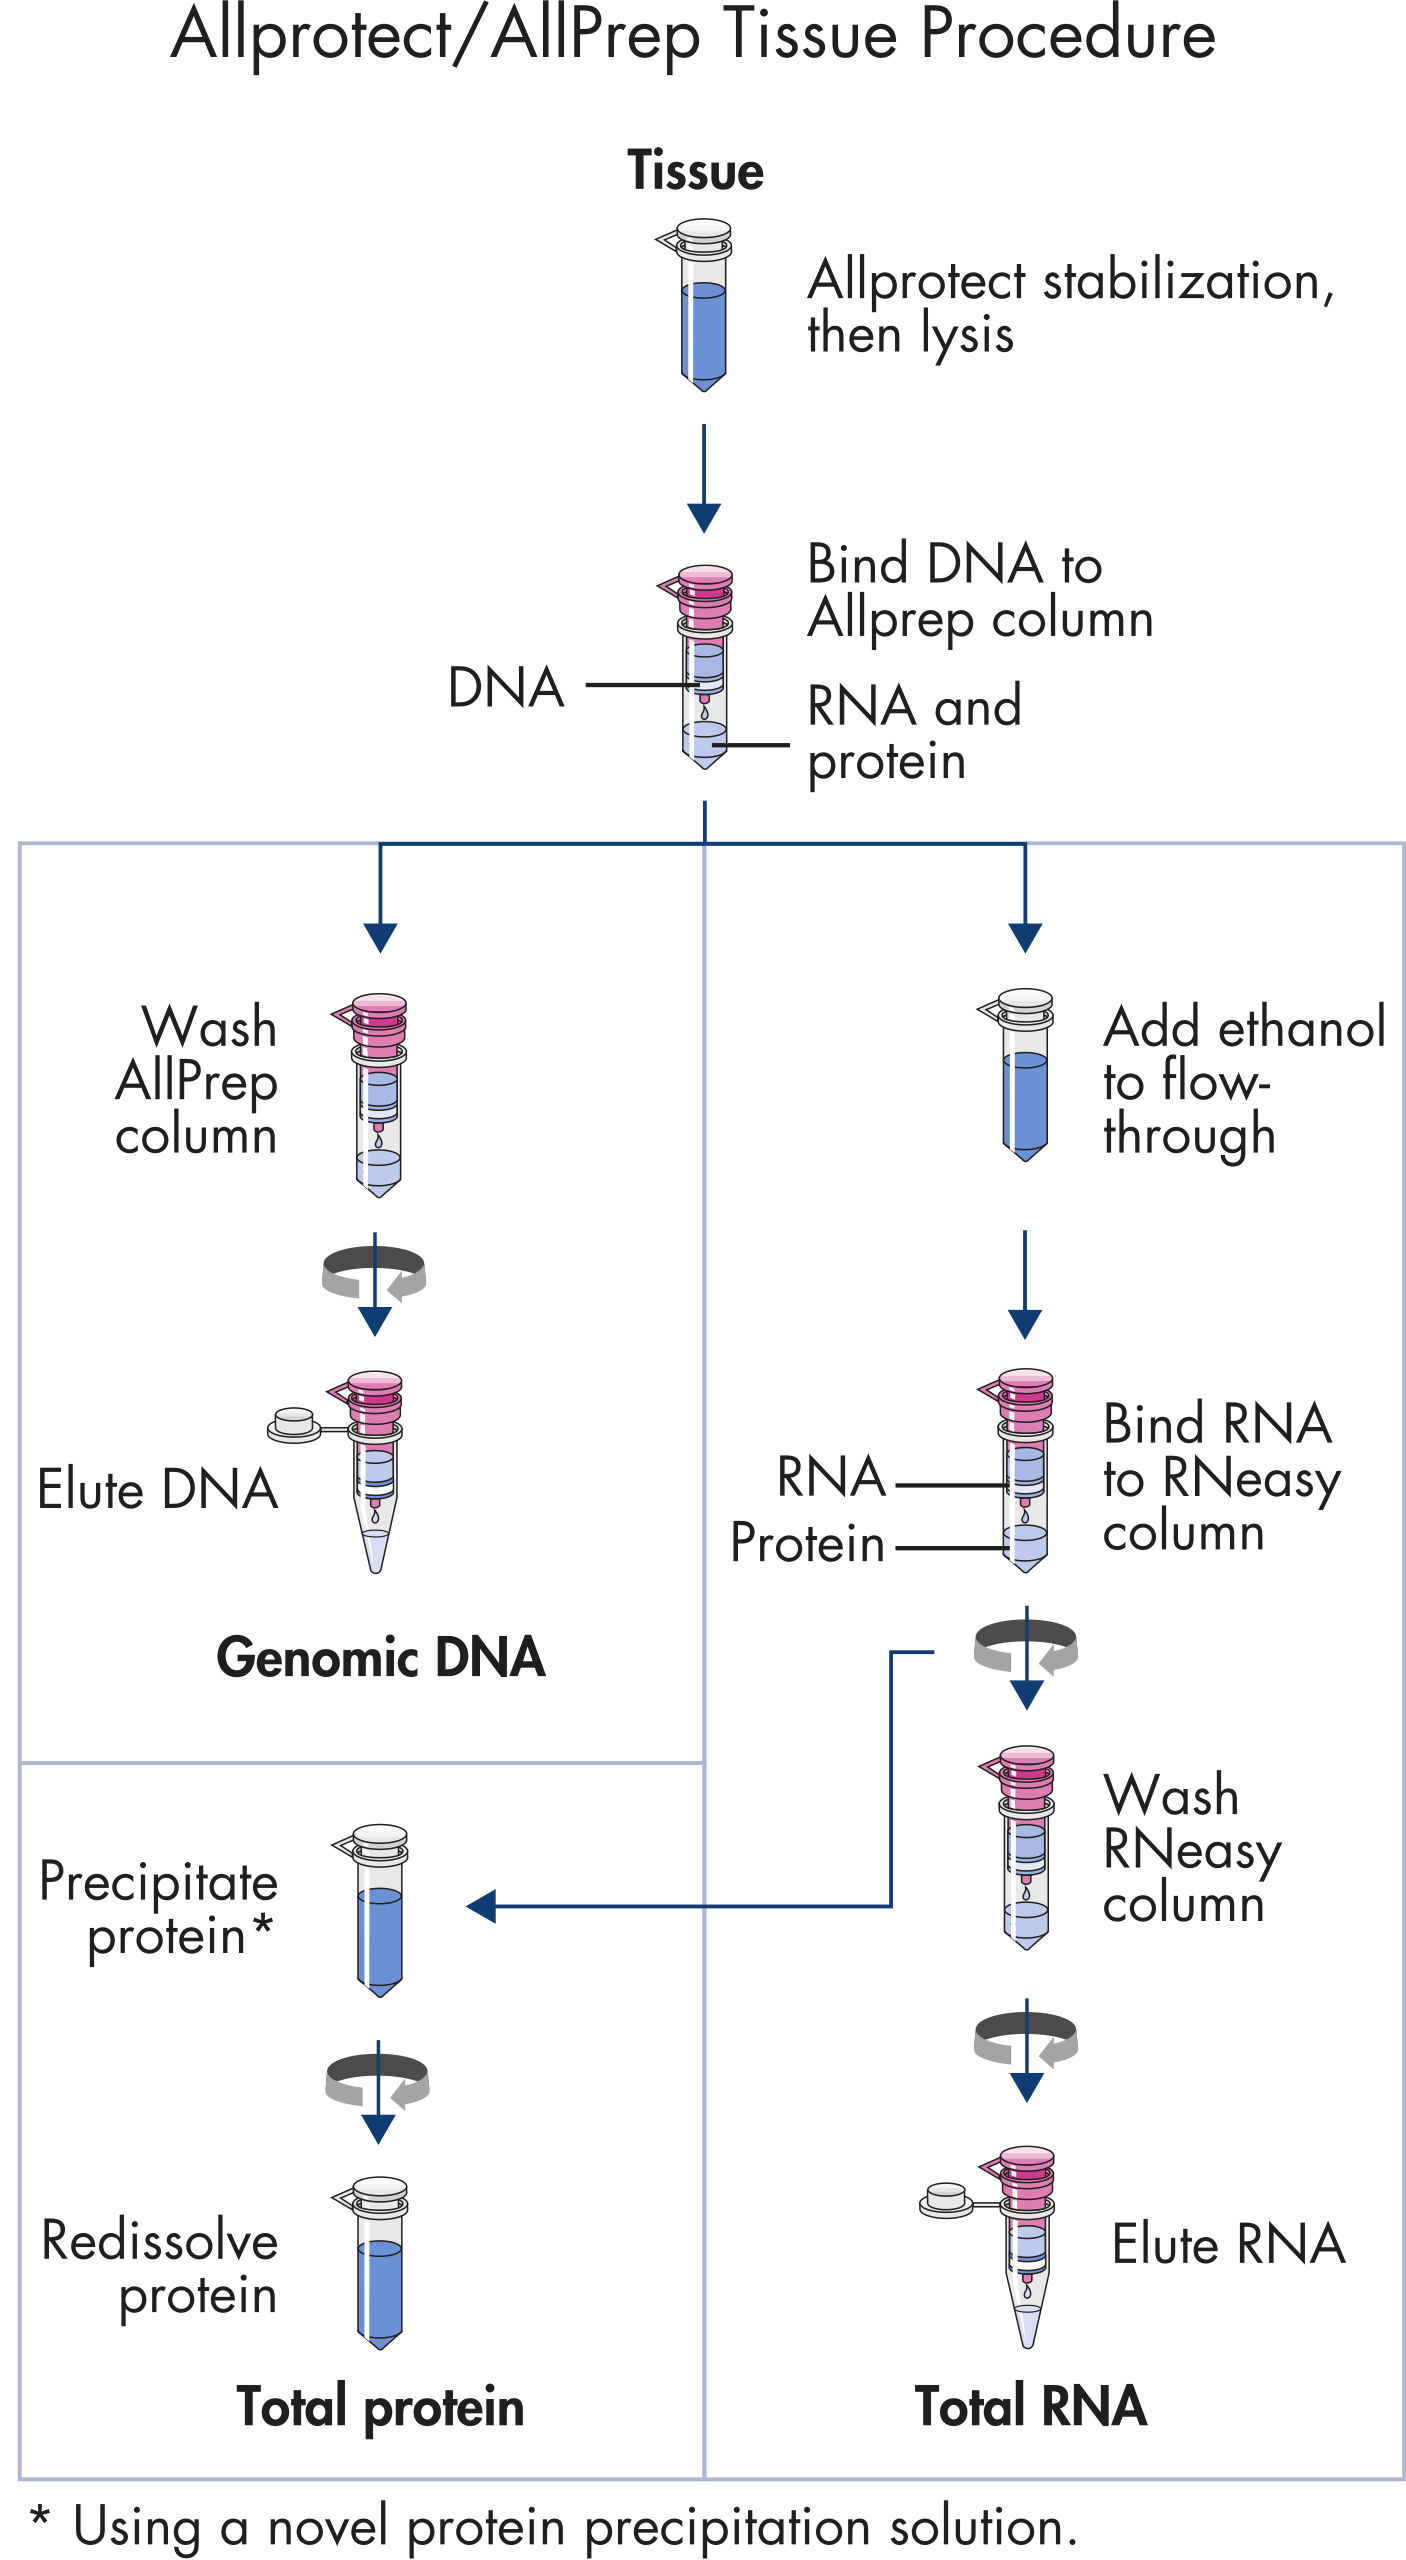
\includegraphics[scale=0.08]{AldoFruc_RNAPurify.jpg}
            \caption{mRNA Purification}
            \label{fig: mRNA Purification}
        \end{subfigure}
        \begin{subfigure}[b]{0.3\textwidth}
            \centering
            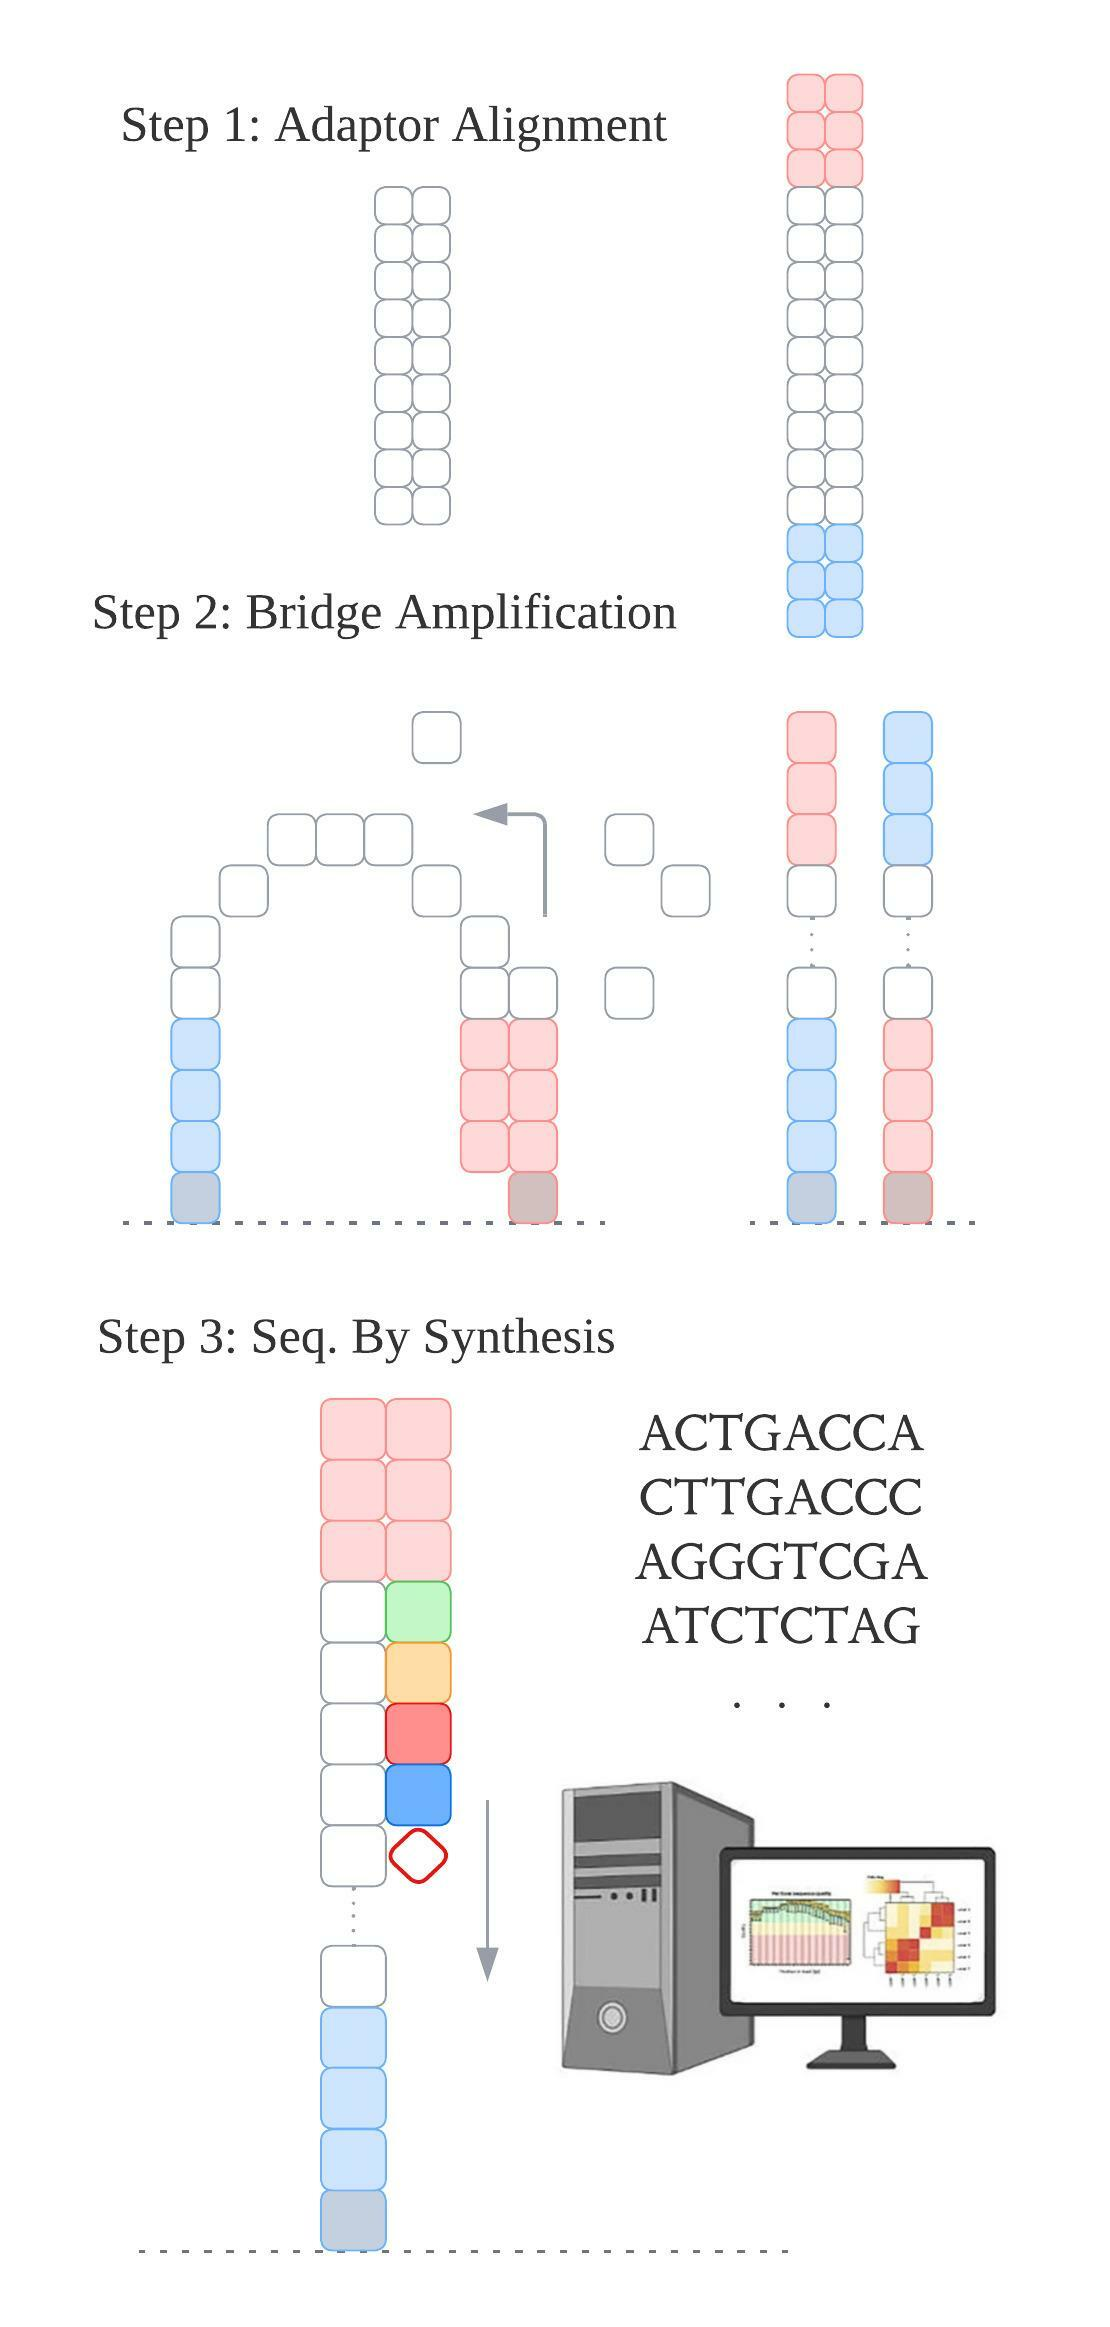
\includegraphics[scale=0.39]{AldoFruc_NGS.jpg}
            \caption{Next-Generation Sequencing \cite{boldogkHoi2019long}}
            \label{fig: NGS}
        \end{subfigure}
        \renewcommand{\figurename}{Figure 2}
           \caption{The workflow of mRNA data collection and processing}
           \label{fig: The workflow of sample collection}
   \end{figure}
\end{frame}

\begin{frame}
    \framesubtitle{Methodology: Sequence Alignment}
    \vspace{-20px}
    \begin{figure}[h]
        \renewcommand{\figurename}{Figure 3}
        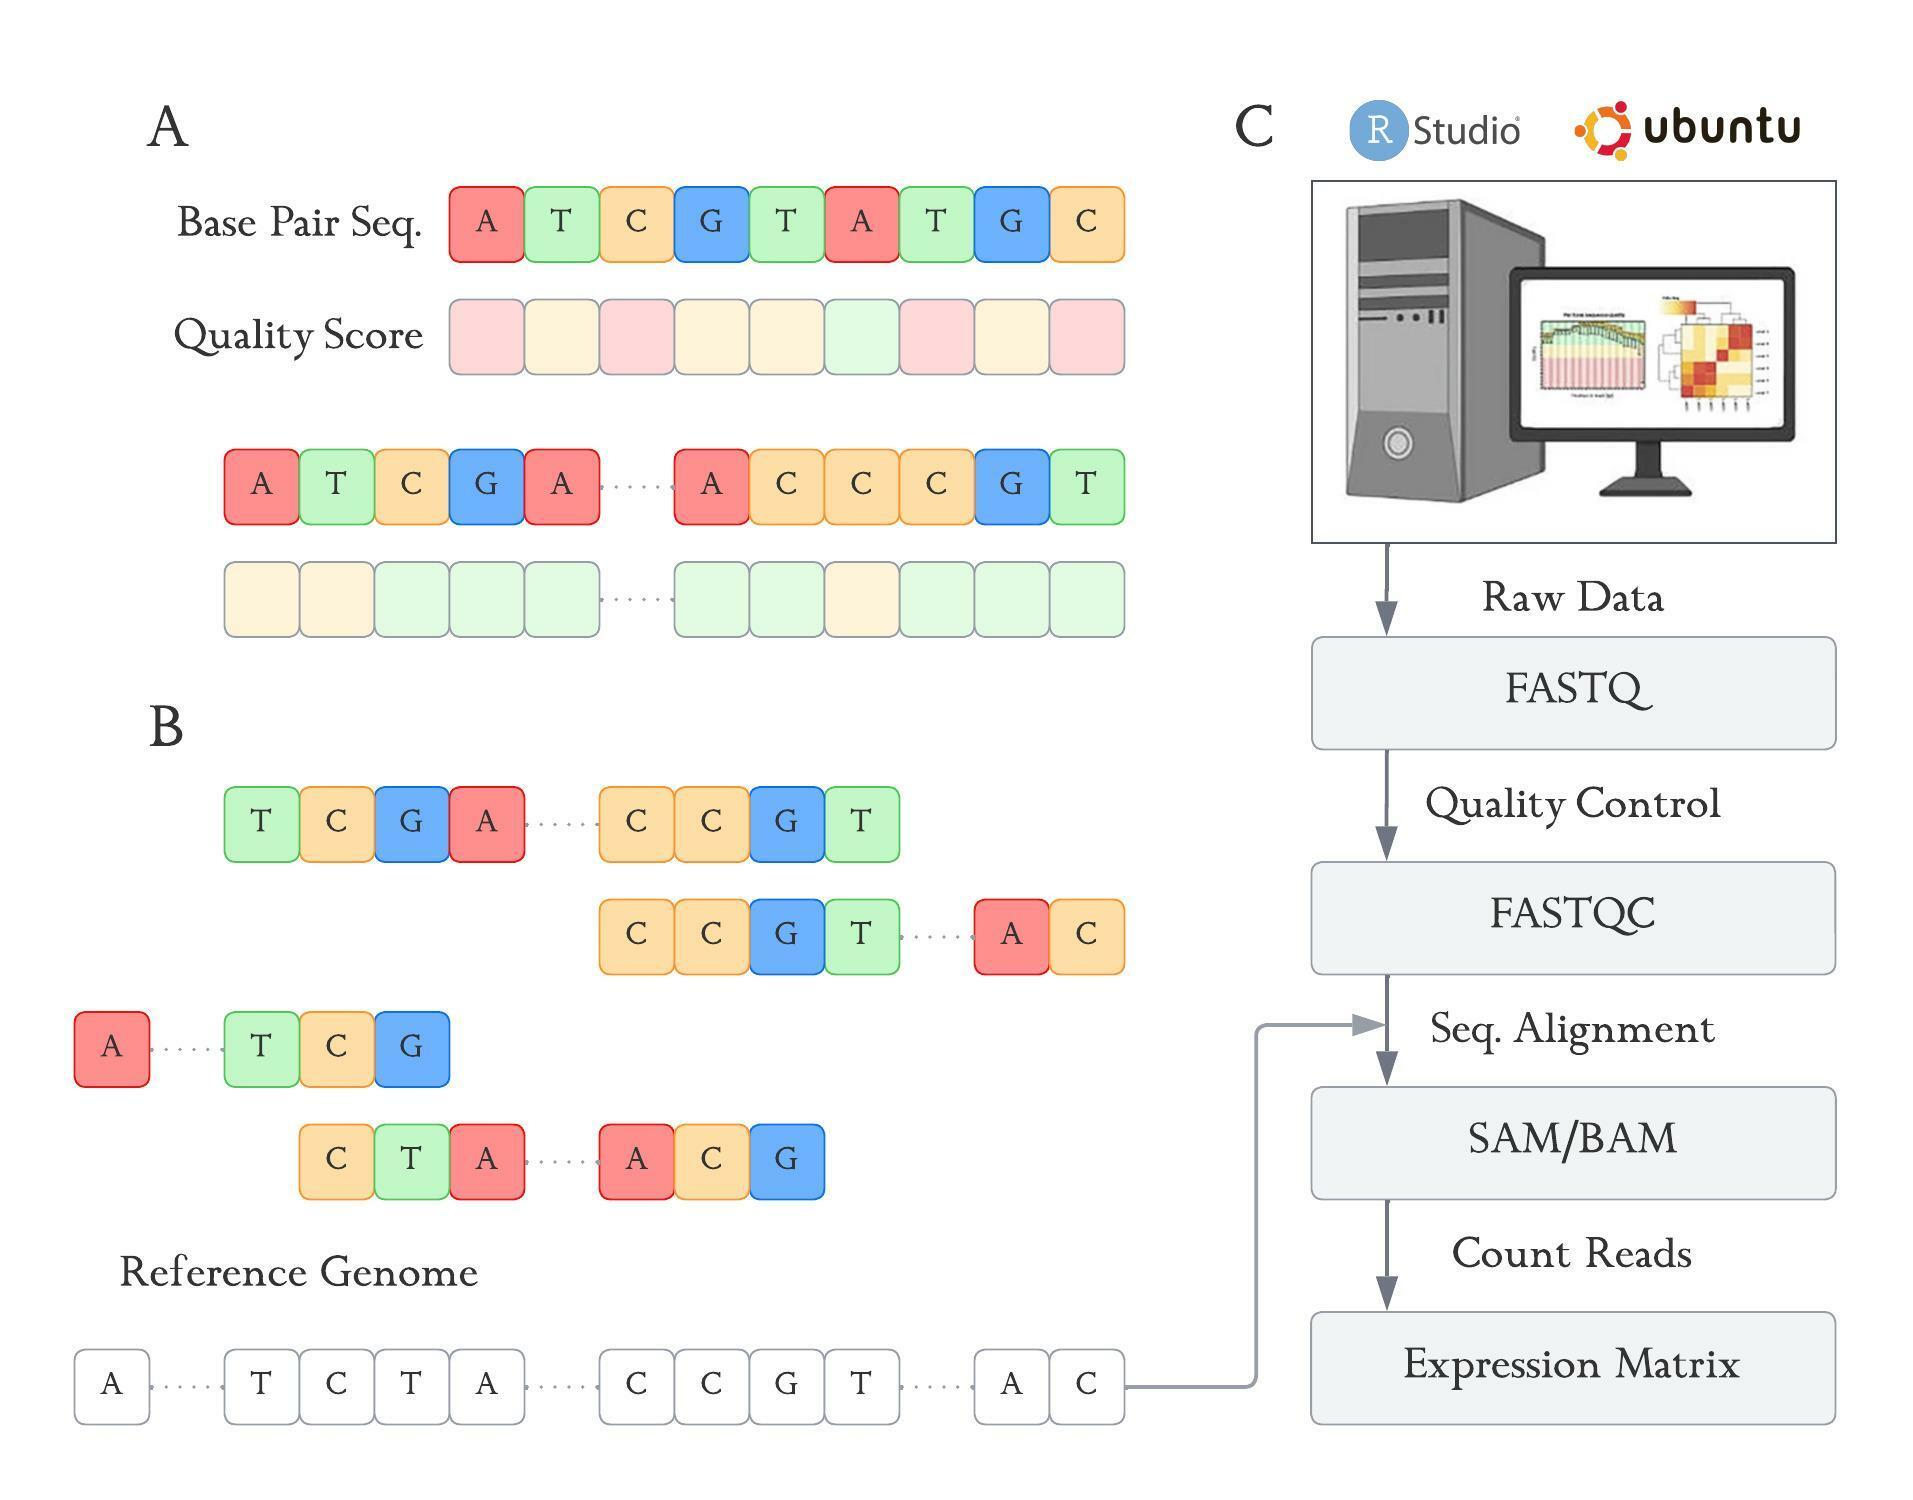
\includegraphics [scale=0.7] {AldoFruc_BioInfo.jpg} 
        \captionsetup{justification=centering}
        \caption{The workflow of Next-Generation Sequencing alignment \\ (\textbf{a}) Trim the Raw Data (\textbf{b}) Sequence Alignment (\textbf{c}) Processed File Generation}
    \end{figure}
\end{frame}

\begin{frame}
    \framesubtitle{Methodology: Matrix Normalization}
    \vspace{-20px}
    \begin{figure}[h]
        \renewcommand{\figurename}{Figure 4}
        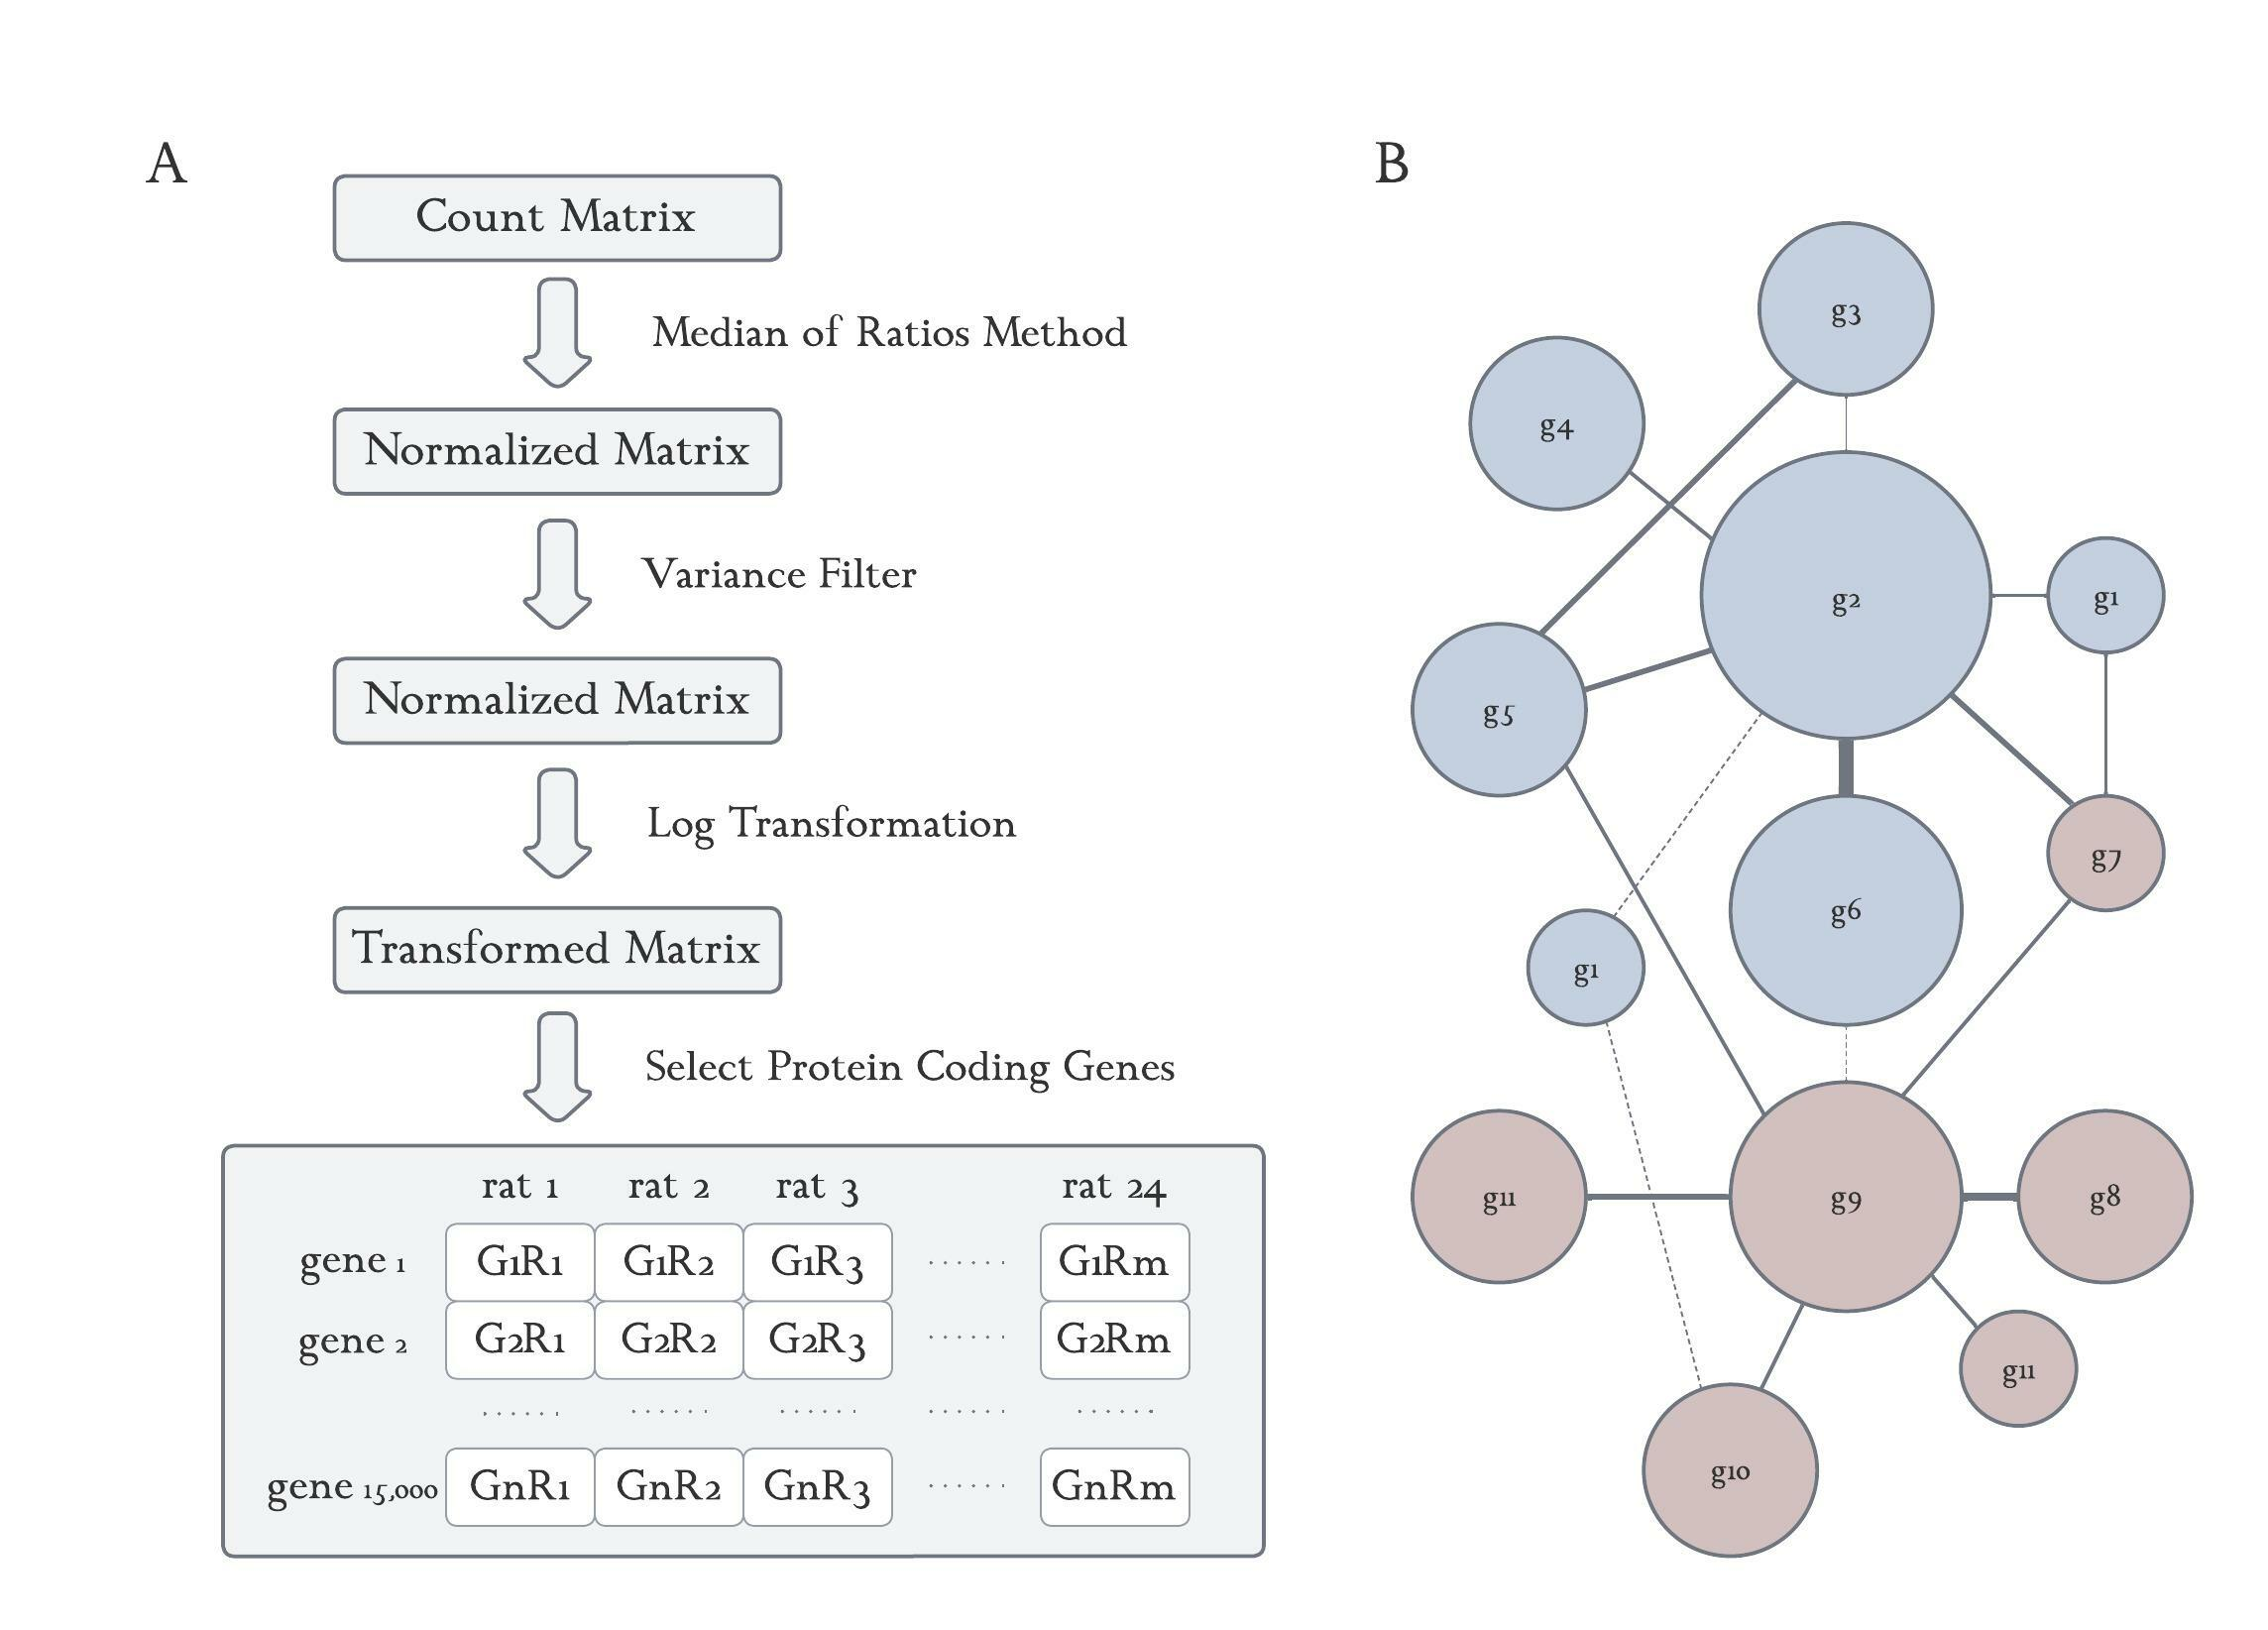
\includegraphics [scale=0.68] {AldoFruc_DataProcess.jpg} 
        \captionsetup{justification=centering}
        \caption{The workflow of matrix data processing (\textbf{a}) Data cleaning (\textbf{b}) Gene Co-expression Network}
    \end{figure}
\end{frame}

\begin{frame}
    \framesubtitle{Methodology: WCGNA I - Weighted Correlation Matrix}
    \begin{columns}[T,onlytextwidth]
        \column{0.5\textwidth}
            \begin{itemize}
                \item Weighted Correlation Network Analysis (\textbf{WGCNA}) \cite{langfelder2008wgcna}\cite{zhang2005general}
                \begin{itemize}
                    \item Cluster Similar Genes
                \end{itemize}
                \item Co-expression Network
                \begin{itemize}
                    \item Vertex: Gene
                    \item Edge: Correlation
                \end{itemize}
                \item Soft Threshold (Power) Selection
                \begin{itemize}
                    \item Scale-Free Network
                    \item Scale Independence
                    \item Connectivity
                \end{itemize}
                \item Adjacency Matrix Generation
                \begin{itemize}
                    \item \texttt{abs(cor(gene1, gene2))}\textsuperscript{\texttt{power}}
                    \item \texttt{(0.5+cor(gene1, gene2)/2)}\textsuperscript{\texttt{power}}
                \end{itemize}

            \end{itemize}
        \column{0.5\textwidth}
        \vspace{-35px}
        \begin{figure}[h]
            \renewcommand{\figurename}{Figure 5}
            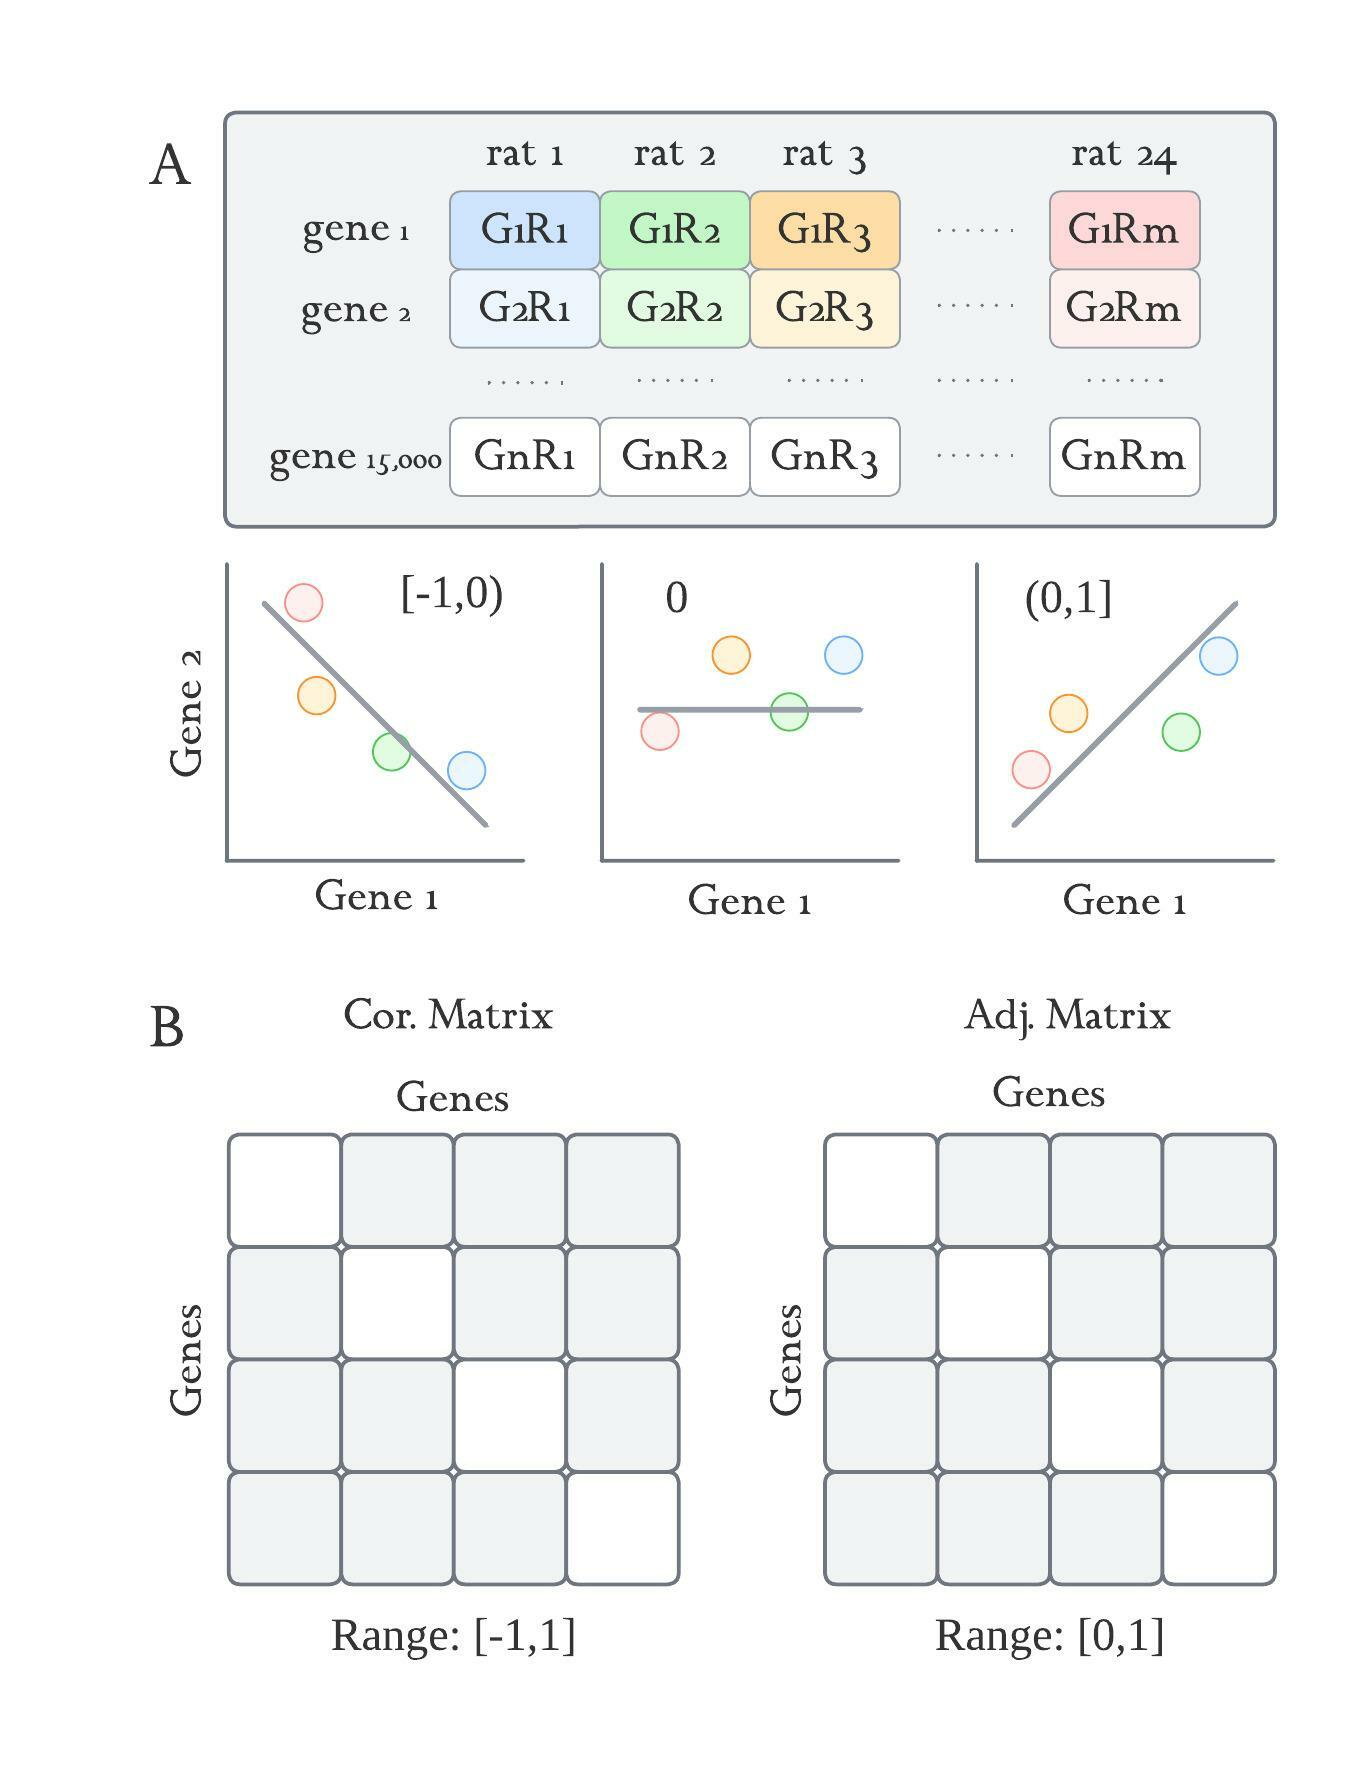
\includegraphics [scale=0.6] {AldoFruc_AdjMatrix.jpg} 
            \captionsetup{justification=centering}
            \caption{The workflow of WGCNA I (\textbf{a}) Correlation calculation (\textbf{b}) Adjacency matrix generation}
        \end{figure}
    \end{columns}
\end{frame}

\begin{frame}
    \framesubtitle{Methodology: WCGNA II - Module Identification}
    \begin{columns}[T,onlytextwidth]
        \column{0.5\textwidth}
            \begin{itemize}
                \item Topological Overlap Measurement (TOM)
                \begin{itemize}
                    \item Measure of Similarity
                    \item $\uparrow \text{Cor}(i,j)$ $\uparrow \text{TOM}(i,j)$ $\downarrow \text{TOM.dissim}(i,j)$
                \end{itemize}
                \item Module Assignment of Genes
                \begin{itemize}
                    \item Hierachical Clustering
                    \item Gene Dendrogram
                \end{itemize}
                \item Module-Trait Relationship
                \begin{itemize}
                    \item Phenotypes, Biological Measurements
                    \item GO Enrichment analysis
                \end{itemize}
            \end{itemize}
        \column{0.5\textwidth}
        \vspace{-35px}
        \begin{figure}[h]
            \renewcommand{\figurename}{Figure 6}
            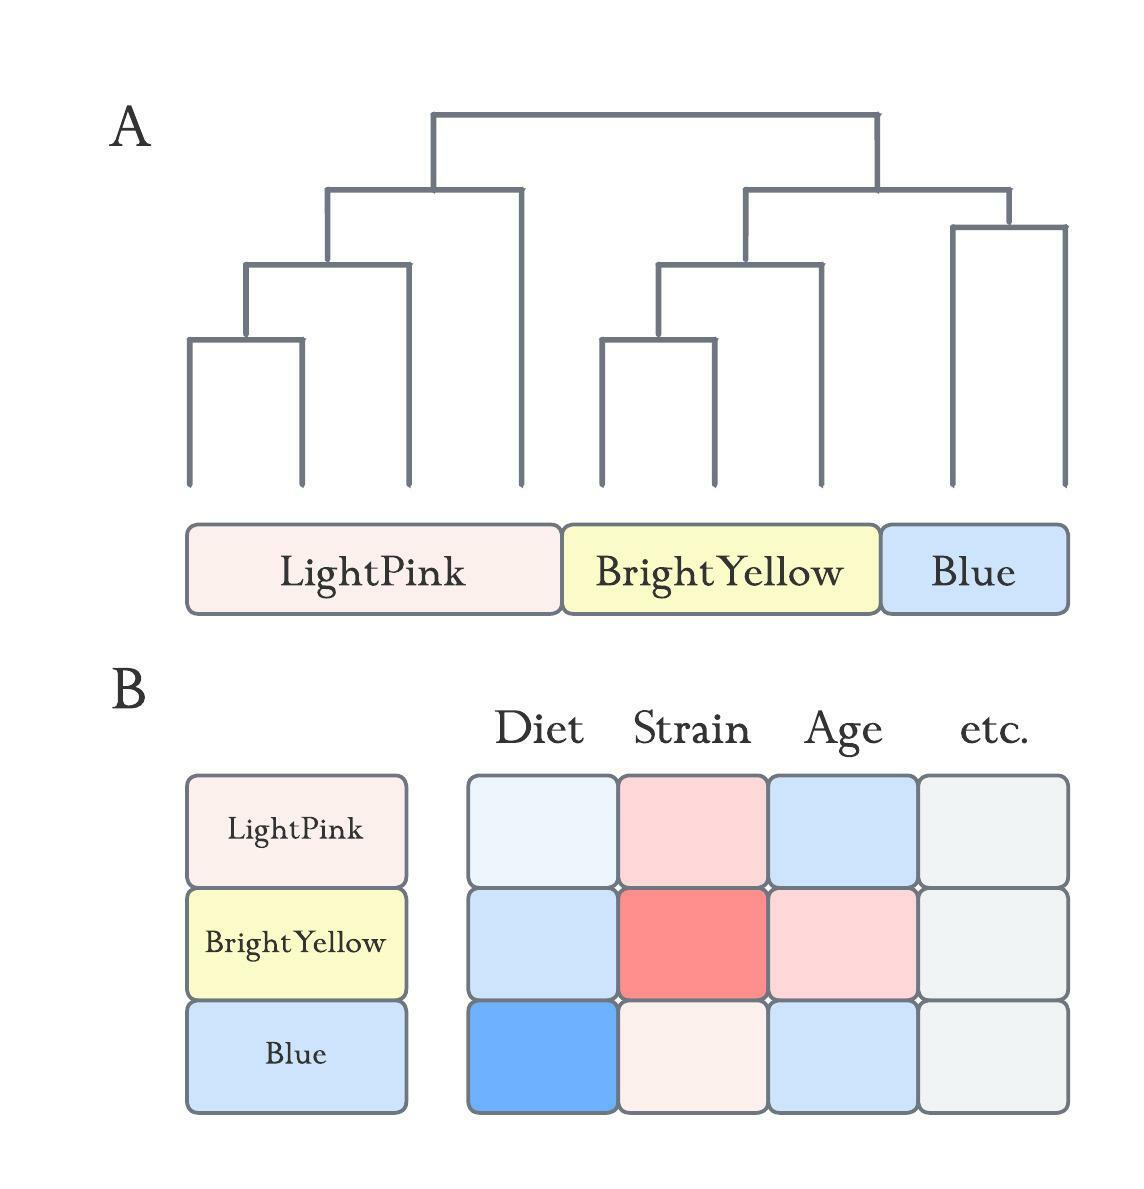
\includegraphics [scale=0.75] {AldoFruc_Module.jpg} 
            \captionsetup{justification=centering}
            \caption{The workflow of WGCNA II (\textbf{a}) Clustering of similar genes (\textbf{b}) Module-Trait Relationship}
        \end{figure}
    \end{columns}
\end{frame}

\subsection{Results}
\begin{frame}
    \framesubtitle{Results: Module Generation}
    \begin{figure}[h]
        \hspace{-30px}
        \renewcommand{\figurename}{Figure 7}
        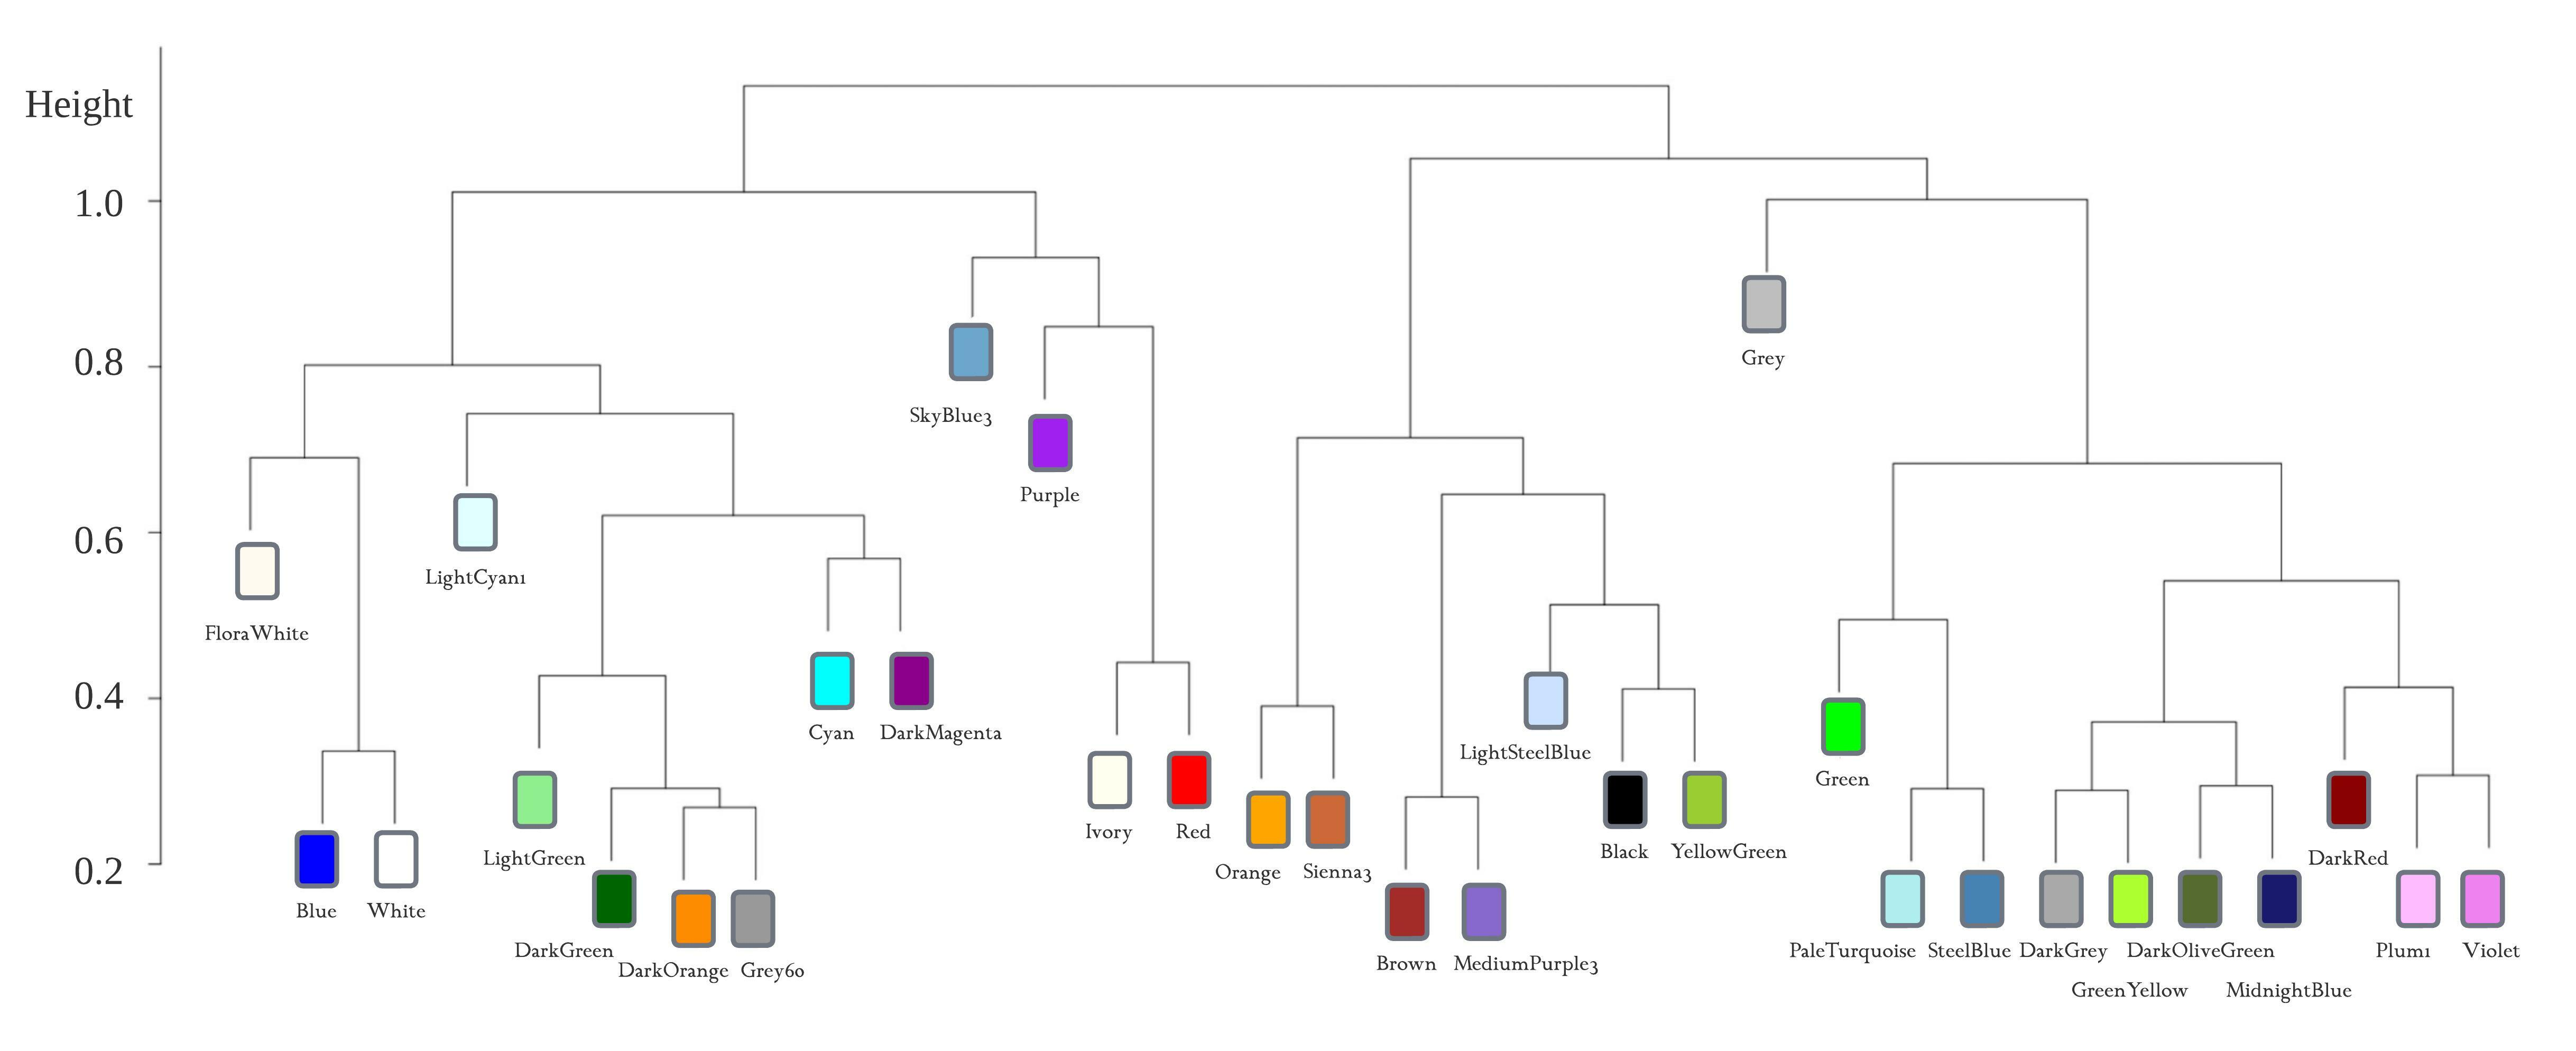
\includegraphics [scale=0.44] {AldoFruc_ModuleResult.jpg} 
        \captionsetup{justification=centering}
        \caption{The 32 gene modules generated using WGCNA}
    \end{figure}
\end{frame}

\begin{frame}
    \framesubtitle{Results: Module Trait Relationship}
        \begin{itemize}
            \item Module Trait Diagram
            \begin{itemize}
                \item correlation index (p-value)
                \item identify expression changes in response to fructose in both groups
            \end{itemize}
        \end{itemize}

        \begin{figure}[h]
            \renewcommand{\figurename}{Figure 8}
            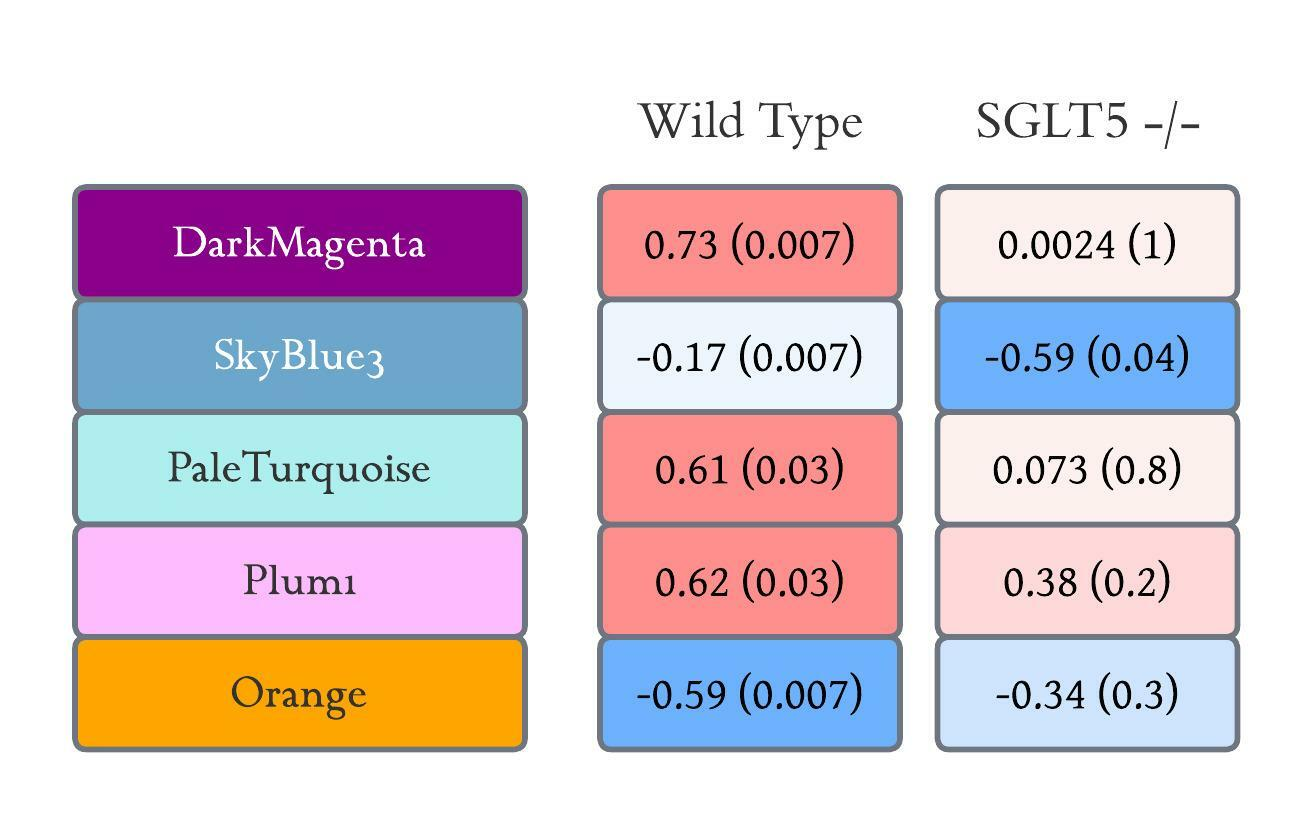
\includegraphics [scale=0.8] {AldoFruc_ModuleTraitResult.jpg} 
            \captionsetup{justification=centering}
            \caption{Selected Module-Trait Relationship diagram}
        \end{figure}
\end{frame}

\begin{frame}
    \framesubtitle{Results: Aldosterone-Related Modules}
    \begin{itemize}
        \item Open source transcriptome (ASDT epithelial cells) \cite{poulsen2018rna}
        \begin{itemize}
            \item 8619 genes mapped to the rat kidney transcriptome
            \item 454 genes significantly changed by Aldosterone
        \end{itemize}
        \item Enrichment Analysis
        \begin{itemize}
            \item 2 modules enriched for aldosterone and correlated with fructose in WT
            \begin{itemize}
                \item Paleturquoise ($\text{p}<3x10^{-2}$) \& Orange ($\text{p}<4x10^{-2}$)
            \end{itemize}
            \item Paleturquoise: Genes involved in Na, Cl and $\text{HCO}_{3}^{-}$ transport
            \begin{itemize}
                \item Scnn1a, ENaC
                \item Slc12a3, NCC
            \end{itemize}
        \end{itemize}
        \item \textbf{Conclusion:} \textit{On a high-salt diet, kidneys from rats given fructose present higher transcriptional activation of aldosterone-responsive genes than those given glucose.}
    \end{itemize}
\end{frame}

\subsection{Works To be Continued}
\begin{frame}
    \begin{itemize}
        \item to further explore the transcriptome
        \item to identify the specific pathways regulated by aldosterone
        \item to conduct quantitative biological experiments if necessary
    \end{itemize}
\end{frame}

%% Part II: COMPUTATIONAL NEUROSCIENCE ----------
\makepart{Computational Neuroscience}

%%% Significance of Computational Neuroscience
\begin{frame}{Why Computational Neuroscience and Neural Engineering?}{Significance of Projects}
    \begin{itemize}
        \item A new approach to interact with tools
        \item Possibility of rehabilitation after severe impairments and discorders
        \item Insights to the brain function and even other subjects
        \begin{figure}[h]
            \renewcommand{\figurename}{Figure 9}
            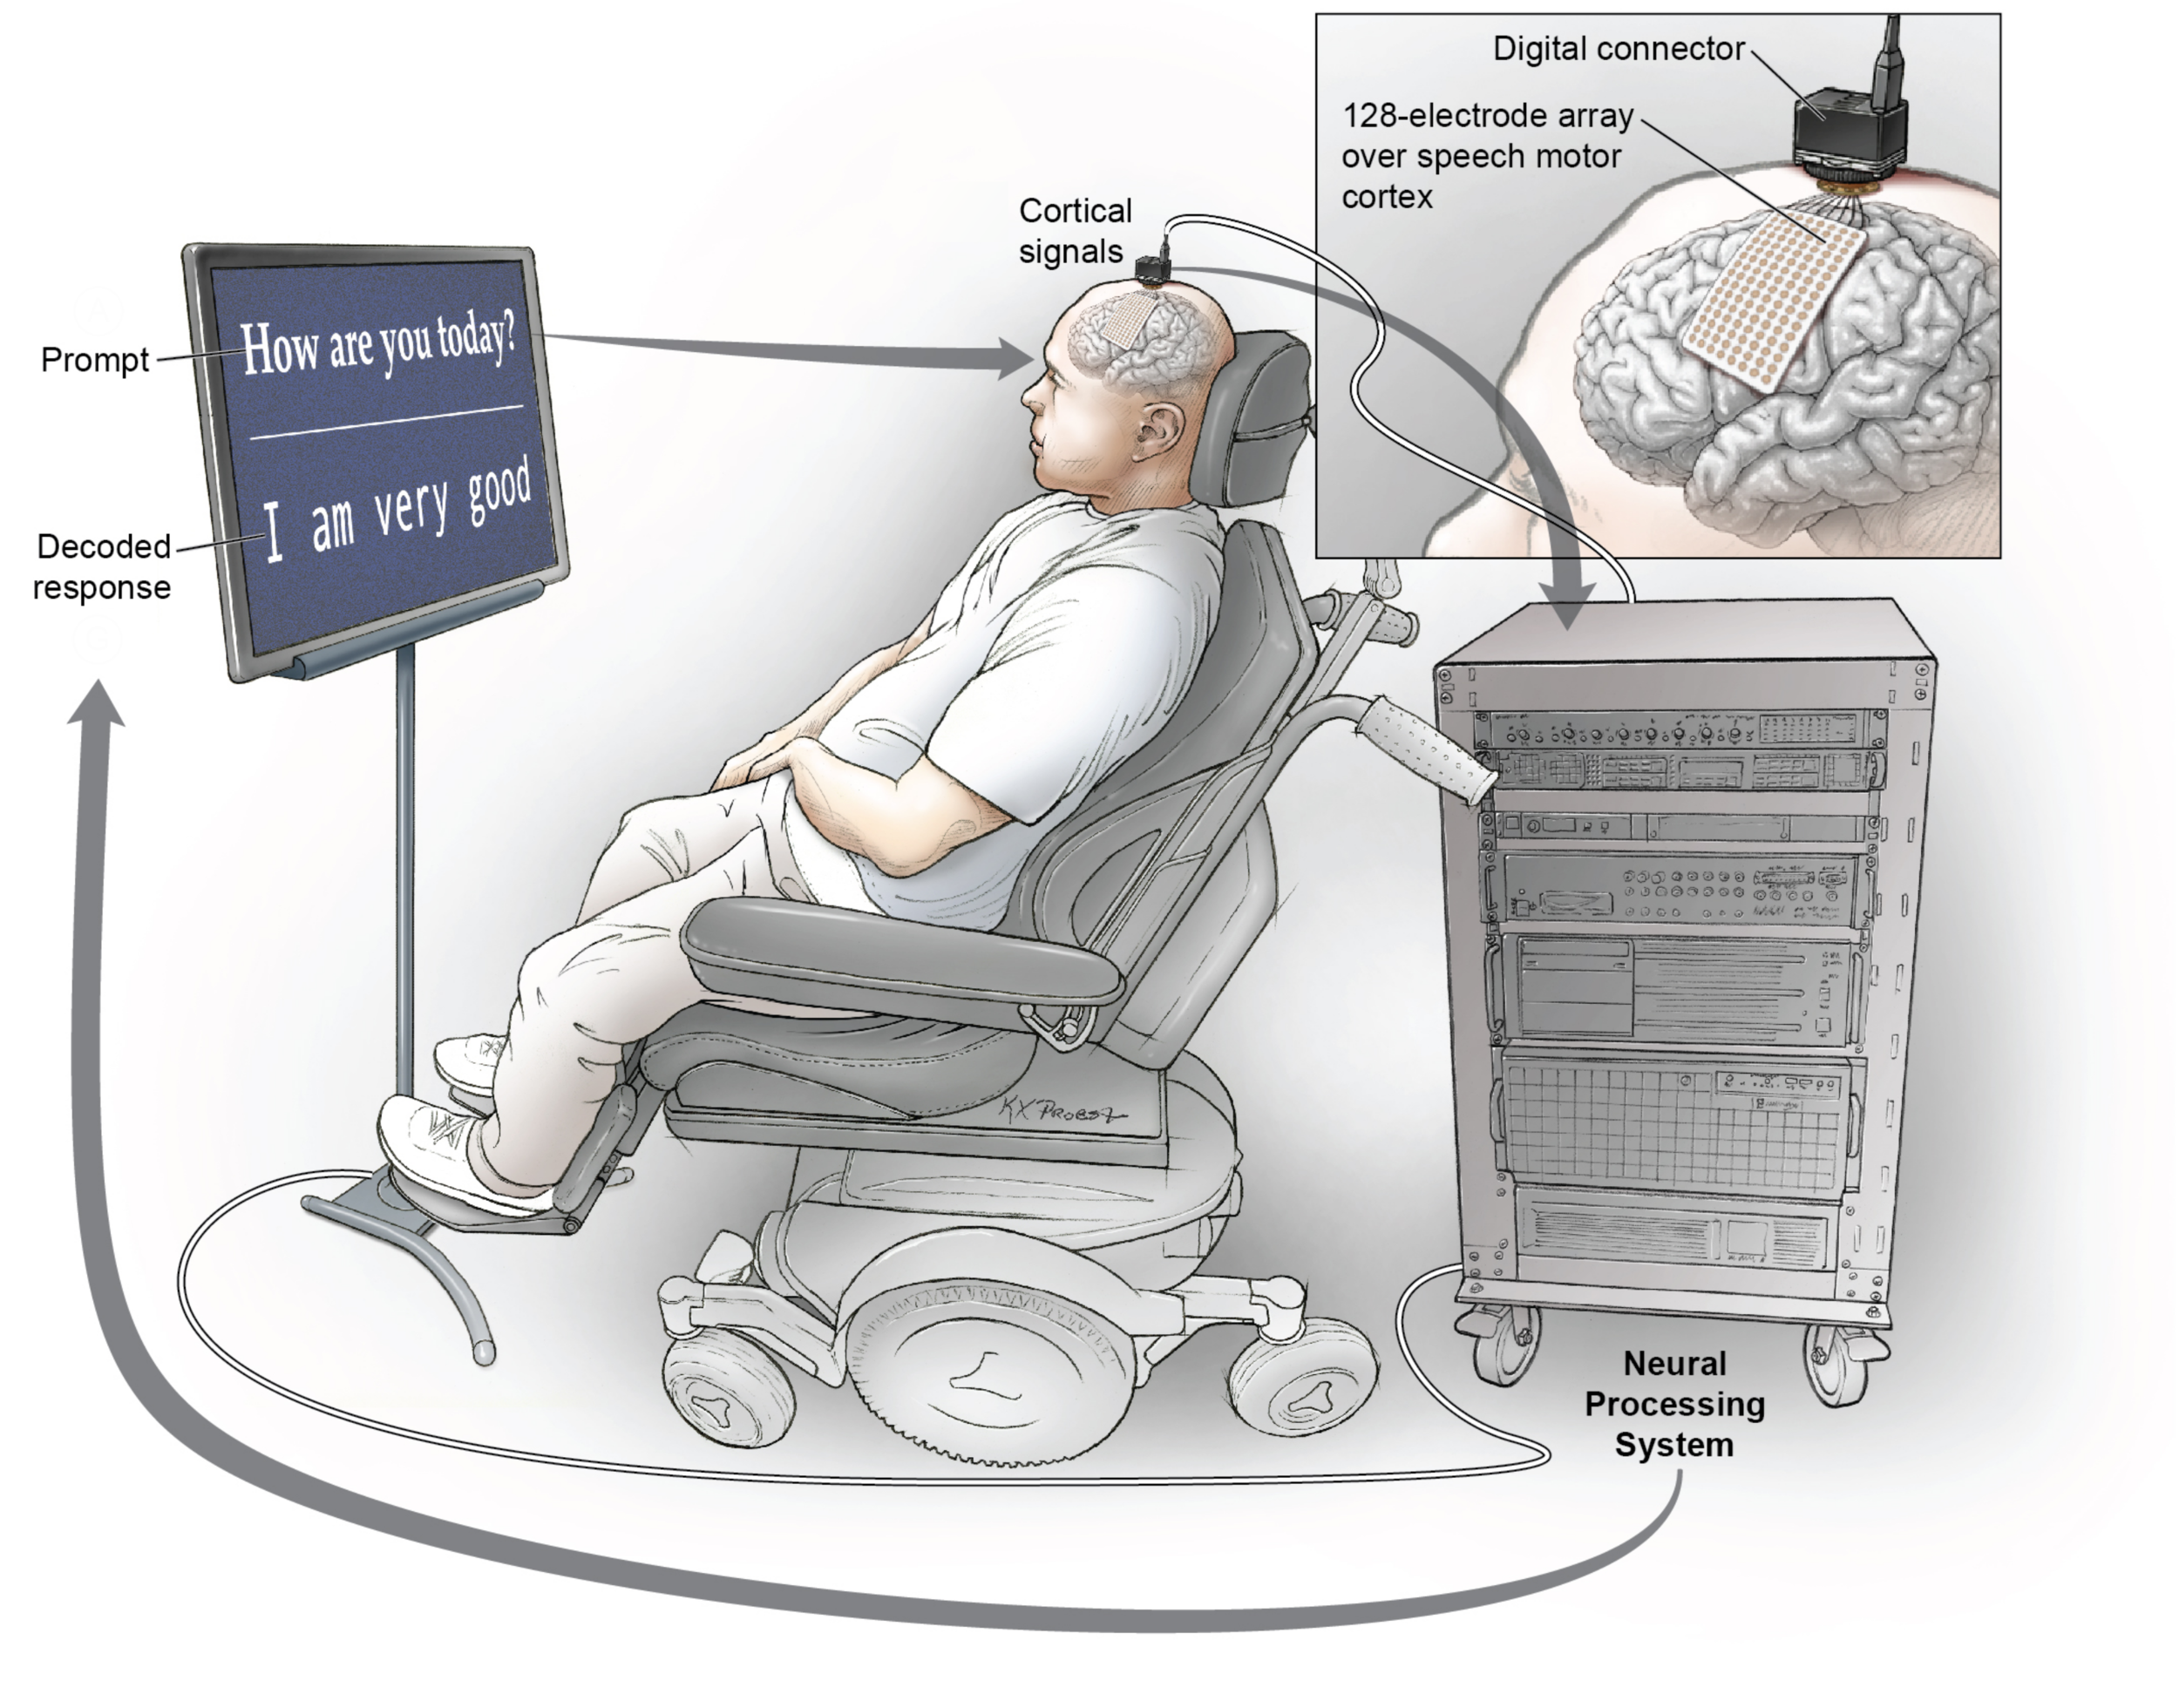
\includegraphics [scale=0.6] {Neuro_BCI.jpg} 
            \captionsetup{justification=centering}
            \caption{Brain-Computer Interface to restore patients' voice \cite{changlabfig}}
        \end{figure}
    \end{itemize}
\end{frame}

%%% Bensmaia Project 1: Neural Basis of Fingertip Biomechanics
\section{Neural Basis of Fingertip Biomechanics}
\begin{frame}{}{Contribution}
\begin{itemize}
    \item \textbf{Duration:} 
    \begin{itemize}
        \item May 2022 - August 2022
    \end{itemize}
    \item \textbf{Keywords:} 
    \begin{itemize}
        \item Computational Neuroscience; Tactile Afferent Receptors
    \end{itemize}
    \item \textbf{Publication:} 
    \begin{itemize}
        \item Unknown
    \end{itemize}
    \item \textbf{Involvement:}
    \begin{itemize}
        \item Data analysis and interpretation
        \item Dissemination and presentation of results
    \end{itemize}
\end{itemize}
\end{frame}

\subsection{Introduction}
\begin{frame}
    \begin{itemize}
        \item Tactile perception of glabrous skin: 4 Mechanoreceptors 
        \item What is the effect of Fingertip Biomechanics?
        \item What about Fingertip on a compliant texture?
    \end{itemize}
    \begin{figure}
        \centering
        \begin{subfigure}[b]{0.3\textwidth}
            \centering
            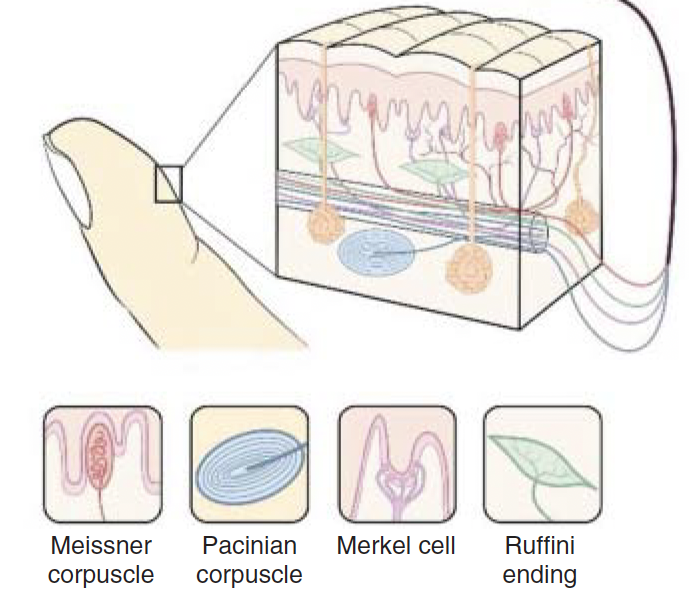
\includegraphics[scale=0.38]{Neuro_RecepLoca.jpg}
            \caption{Mechanoreceptor Location \cite{wixted2018stevens}}
        \end{subfigure}
        \begin{subfigure}[b]{0.3\textwidth}
            \centering
            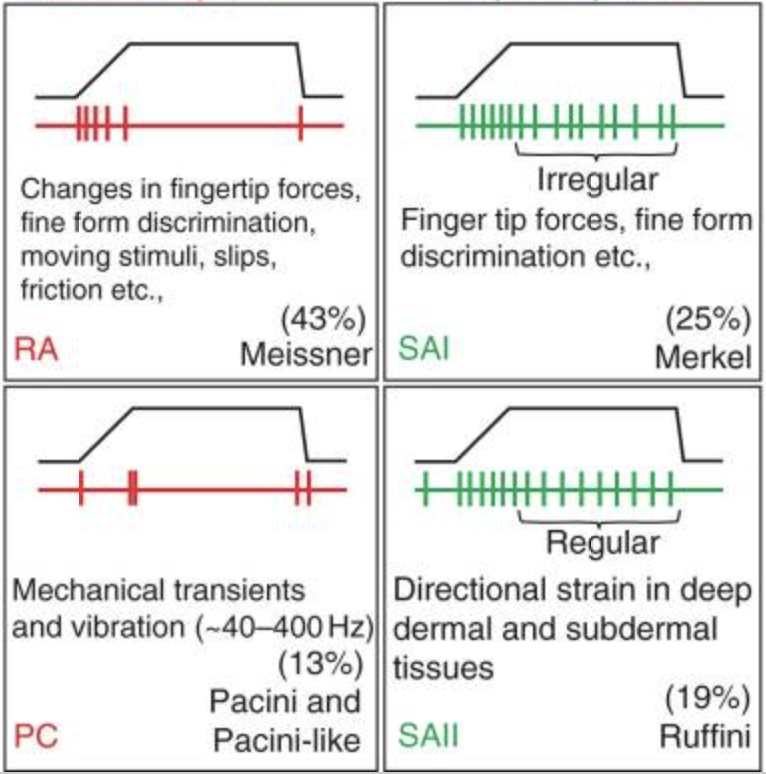
\includegraphics[scale=0.3]{Neuro_RecepFunc.jpg}
            \caption{Mechanoreceptor Functions \cite{delhaye2018neural}}
        \end{subfigure}
        \begin{subfigure}[b]{0.3\textwidth}
            \centering
            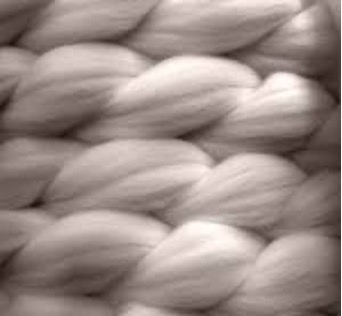
\includegraphics[scale=0.37]{Neuro_Fabric.jpg}
            \caption{Fabric Pattern of Wool Yarn}
        \end{subfigure}
        \renewcommand{\figurename}{Figure 10}
        \caption{Introduction to afferent mechanoreceptors of tactile perception}
    \end{figure}
\end{frame}

\subsection{Methodology}
\begin{frame}
    \framesubtitle{Methodology: Height Map Generation}
    \vspace{-10px}
    \begin{itemize}
        \item Scanning of raw heights and "skin indentation" for frequency analysis
        \item Light refraction and artifacts introduced by scanning
    \end{itemize}
    \begin{figure}
        \centering
        \begin{subfigure}[b]{0.6\textwidth}
            \centering
            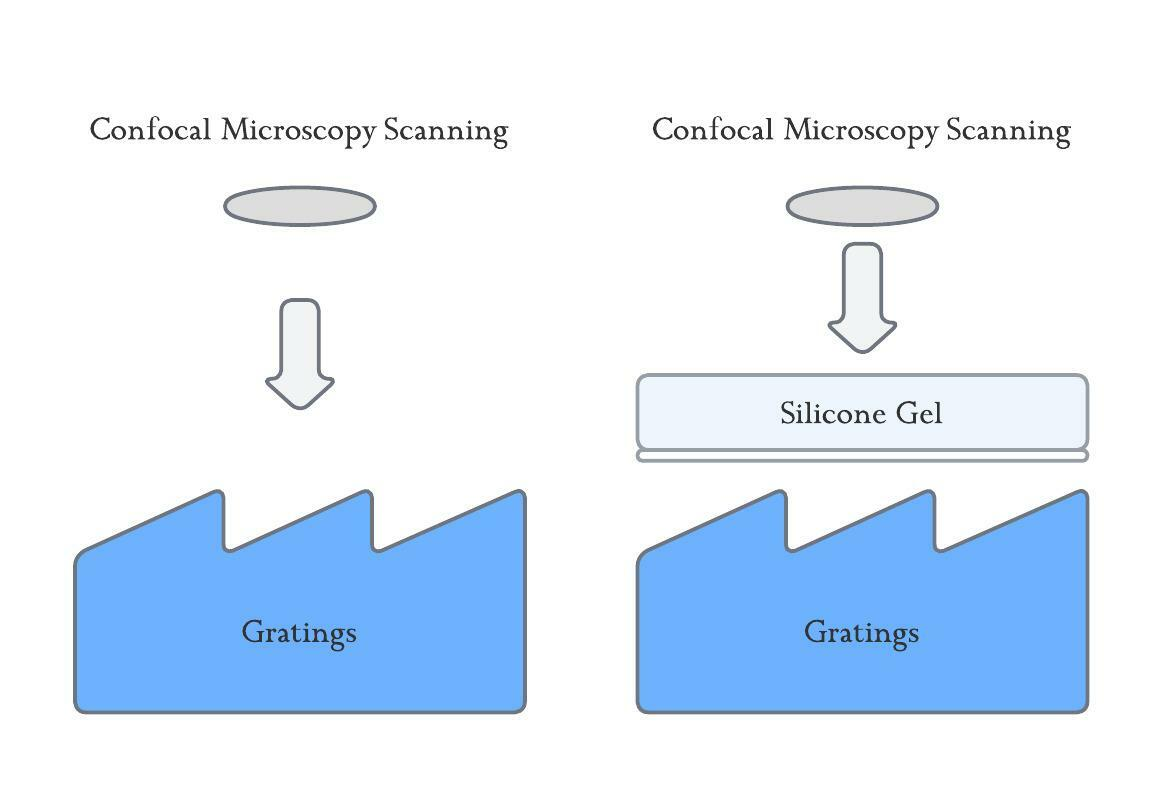
\includegraphics[scale=0.9]{Neuro_Confocal.jpg}
            \caption{Confocal Microscopy Scanning}
        \end{subfigure}
        \begin{subfigure}[b]{0.28\textwidth}
            \centering
            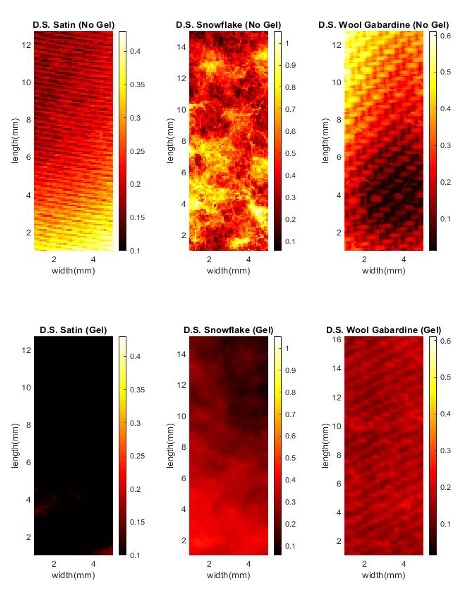
\includegraphics[scale=0.25]{Neuro_RawHeight.jpg}
            \caption{Mechanoreceptor Functions}
        \end{subfigure}
        \renewcommand{\figurename}{Figure 11}
        \caption{Generation of Height Maps}
    \end{figure}
\end{frame}

\begin{frame}
    \framesubtitle{Methodology: Artifact Rejection I}
    \begin{columns}[T,onlytextwidth]
        \column{0.5\textwidth}
            \begin{itemize}
                \item Downsampling
                \begin{itemize}
                    \item Change the resolution of height maps
                \end{itemize}
                \item Detrending
                \begin{itemize}
                    \item Flatten the crease and eliminate artifacts
                \end{itemize}
                \item Force Normalization
                \begin{itemize}
                    \item Noramlize the indentation depth
                \end{itemize}
                \item \textbf{Remaining Problem}
                \begin{itemize}
                    \item Scaling Factors \& Angle Difference
                \end{itemize}
            \end{itemize}
        \column{0.5\textwidth}
            \vspace{-50px}
            \begin{figure}[h]
                \renewcommand{\figurename}{Figure 12}
                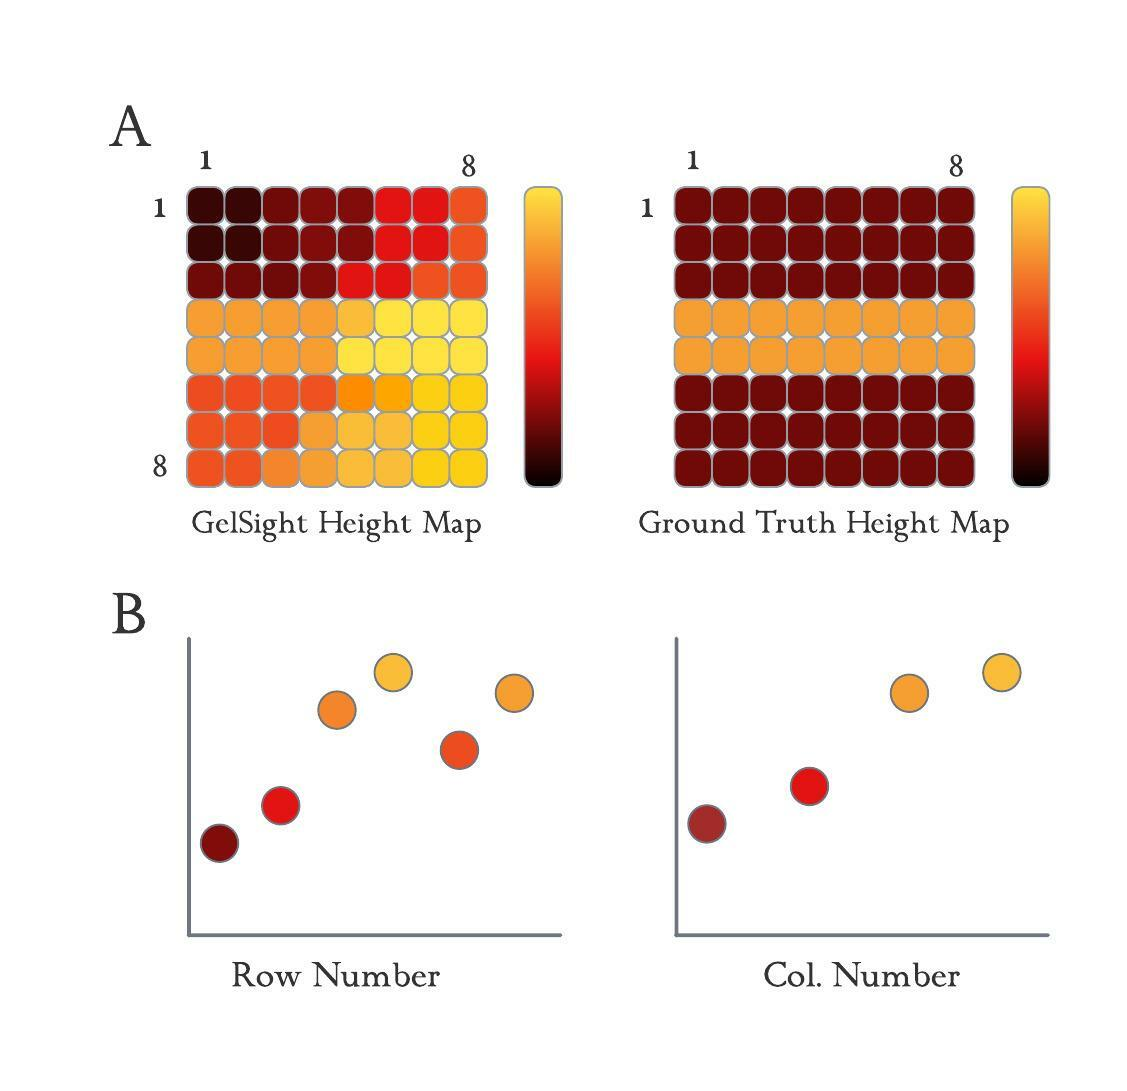
\includegraphics [scale=0.9] {Neuro_Detrending.jpg} 
                \captionsetup{justification=centering}
                \caption{The detrending method (\textbf{a}) Comparison between gelsight and ground truth height map (\textbf{b}) Row-wise and column-wise average height}
            \end{figure}
    \end{columns}
\end{frame}

\begin{frame}
    \framesubtitle{Methodology: Artifact Rejection II}
    \vspace{-15px}
    \begin{itemize}
        \item Matlab-embedded image registration
        \item Cross Correlation of 2 matrix is given by that
         $$\textbf{C}(k,l) = \sum^{M-1}_{m=0}\sum^{N-1}_{n=0}\textbf{X}(m,n)\bar{H}(m-k,n-l)$$, where 
         $-(P-1)\leq k \leq M-1$ and $-(Q-1)\leq l \leq N-1$
    \end{itemize}
    \begin{figure}[h]
        \renewcommand{\figurename}{Figure 13}
        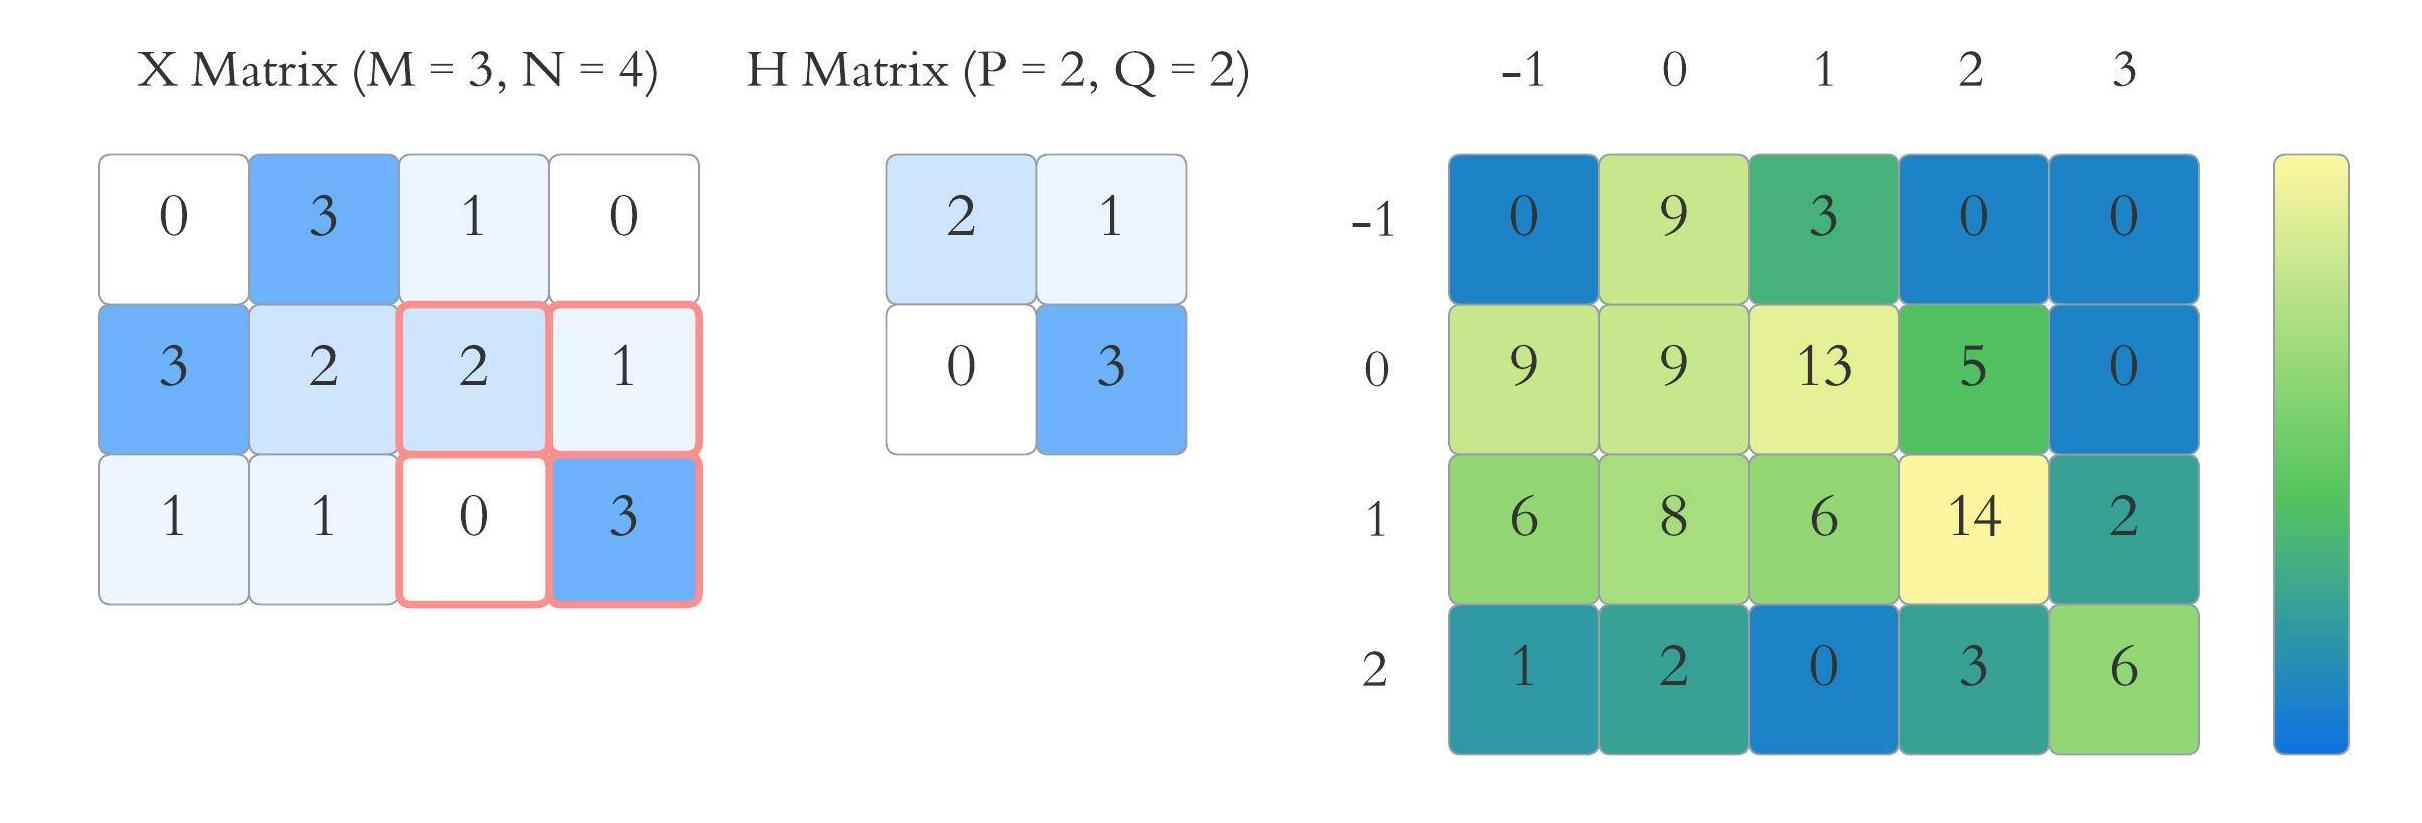
\includegraphics [scale=0.17] {Neuro_CrossCor.jpg} 
        \captionsetup{justification=centering}
        \caption{Example of 2-D cross correlation method of 2 matrices}
    \end{figure}
\end{frame}

\subsection{Results}
\begin{frame}
    \begin{figure}
        \centering
        \begin{subfigure}[b]{0.5\textwidth}
            \centering
            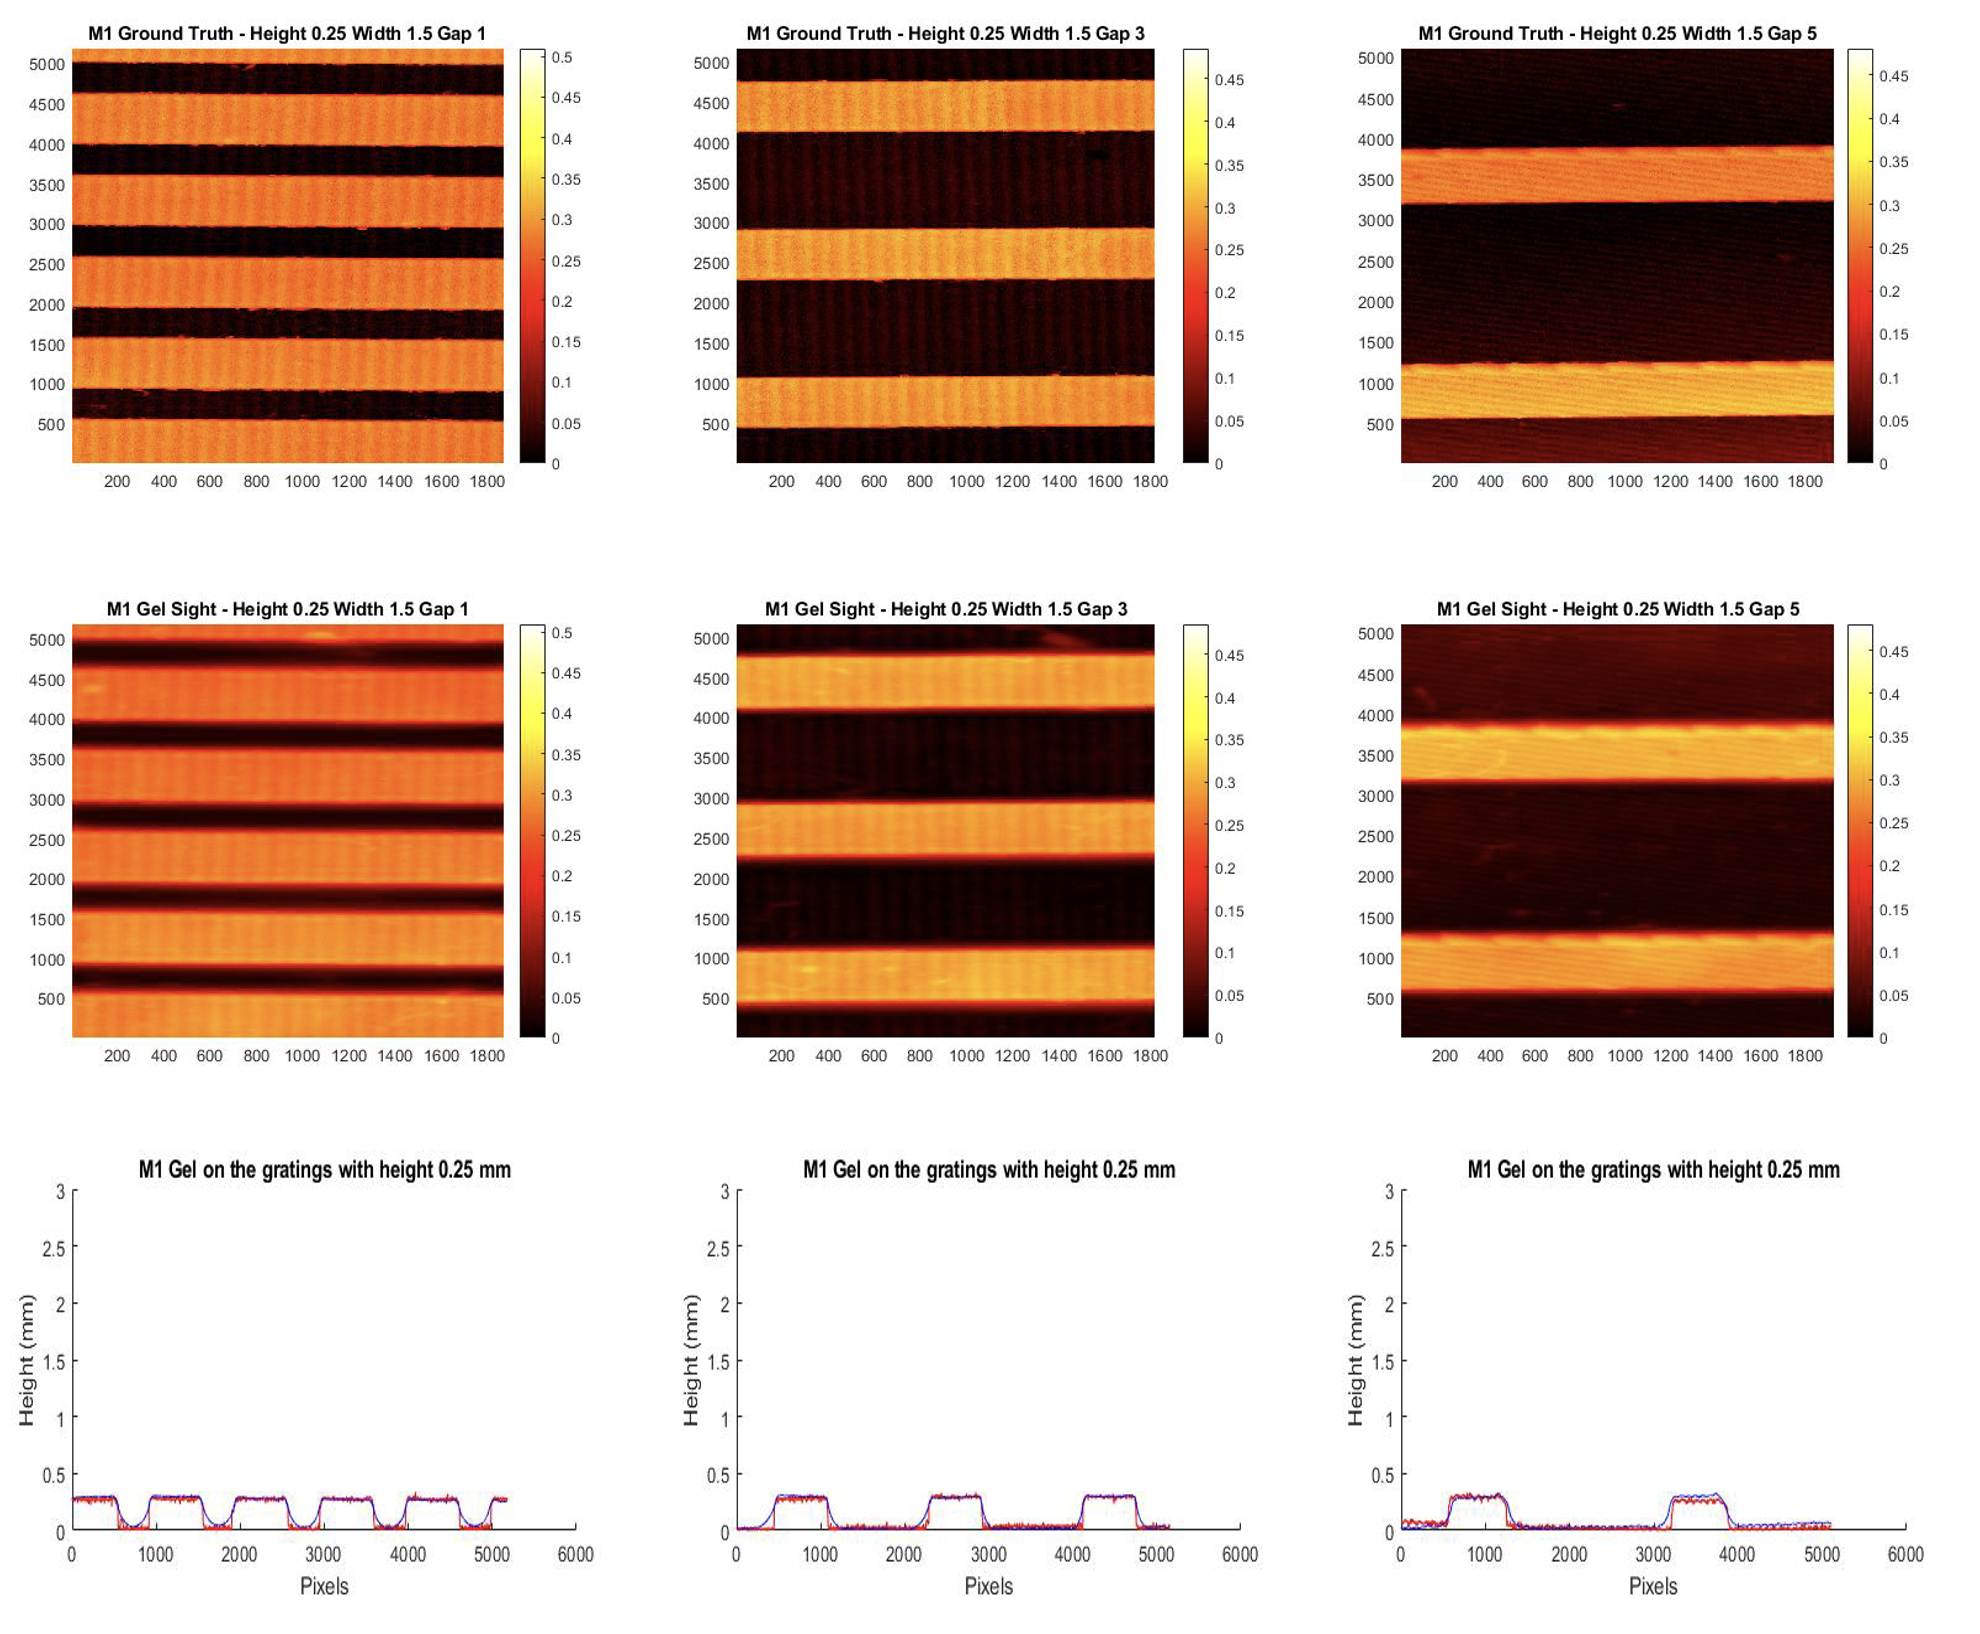
\includegraphics[scale=0.22]{Neuro_ResultGrating.jpg}
            \caption{Aligned Grating Patterns}
        \end{subfigure}
        \begin{subfigure}[b]{0.48\textwidth}
            \centering
            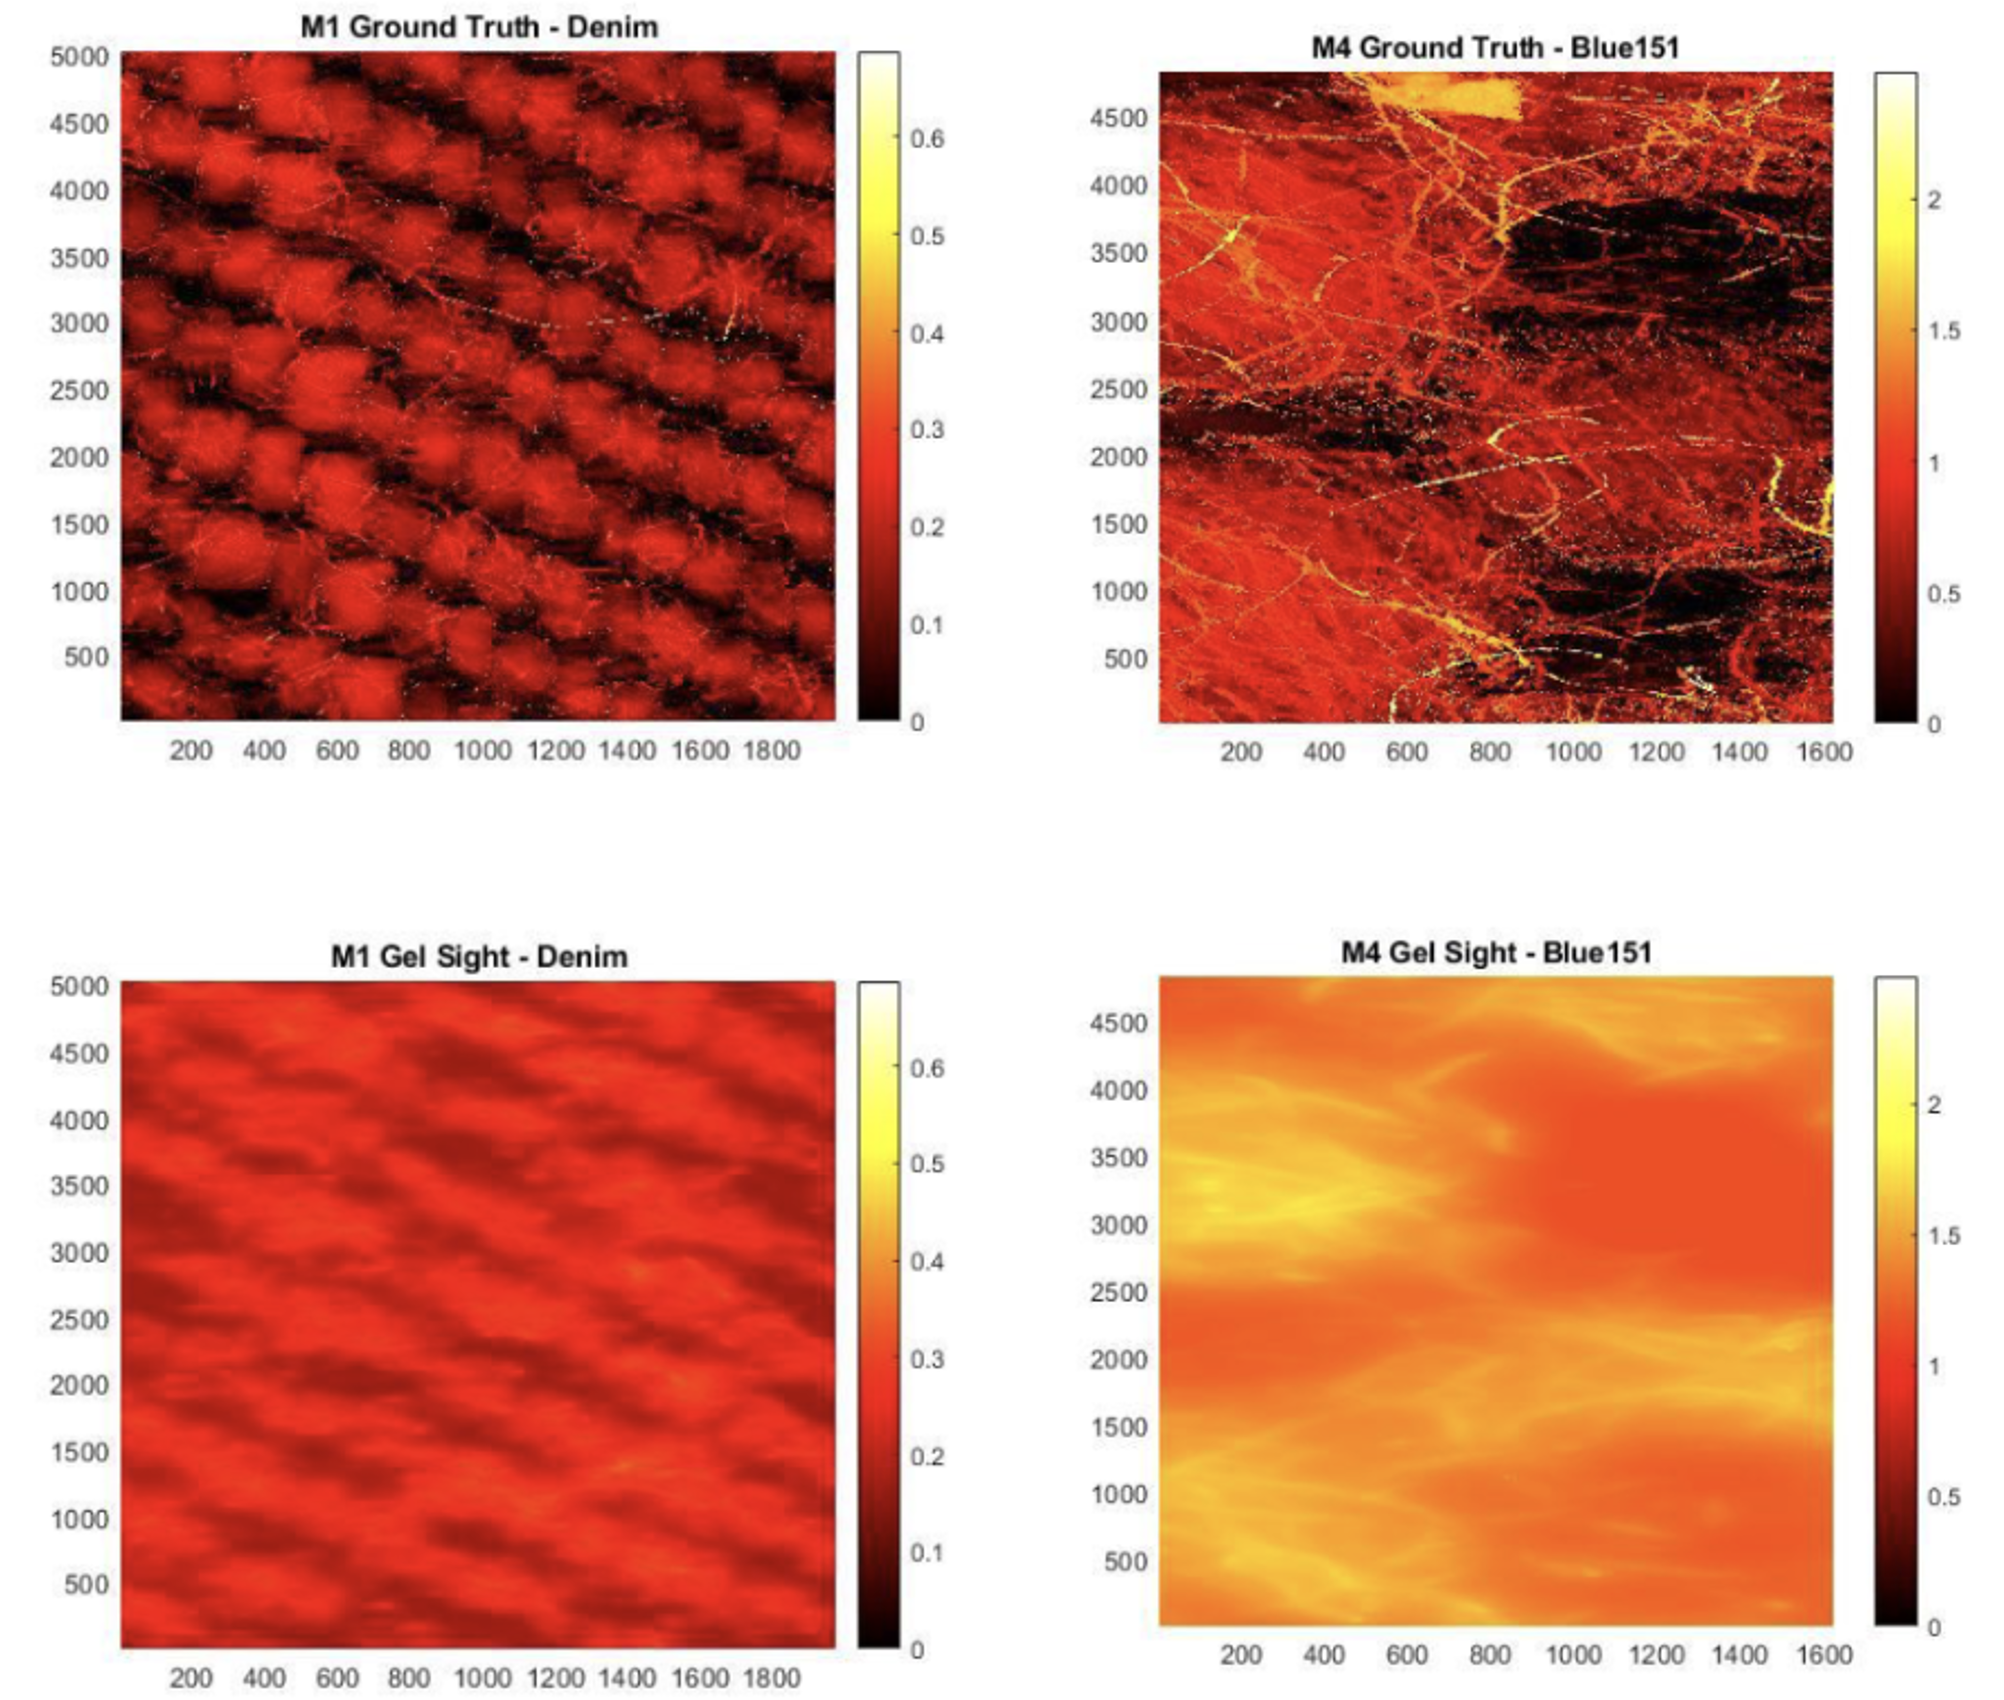
\includegraphics[scale=0.21]{Neuro_ResultFabric.jpg}
            \caption{Aligned Fabric Patterns}
        \end{subfigure}
        \renewcommand{\figurename}{Figure 14}
        \caption{Pixel by pixel alignment of compliant and non-compliant textures}
    \end{figure}
\end{frame}

\begin{frame}[allowframebreaks]{References}
    \printbibliography
\end{frame}
\end{document}